%% LyX 2.3.6.1 created this file.  For more info, see http://www.lyx.org/.
%% Do not edit unless you really know what you are doing.
\documentclass[10pt,english,10pt]{beamer}
\usepackage{lmodern}
\usepackage[T1]{fontenc}
\usepackage[utf8]{inputenc}
\setcounter{tocdepth}{1}
\setlength{\parskip}{\smallskipamount}
\setlength{\parindent}{0pt}
\usepackage{amsbsy}
\usepackage{amstext}
\usepackage{amssymb}
\usepackage{graphicx}
\usepackage[authoryear]{natbib}

\makeatletter
%%%%%%%%%%%%%%%%%%%%%%%%%%%%%% Textclass specific LaTeX commands.
% this default might be overridden by plain title style
\newcommand\makebeamertitle{\frame{\maketitle}}%
% (ERT) argument for the TOC
\AtBeginDocument{%
  \let\origtableofcontents=\tableofcontents
  \def\tableofcontents{\@ifnextchar[{\origtableofcontents}{\gobbletableofcontents}}
  \def\gobbletableofcontents#1{\origtableofcontents}
}

%%%%%%%%%%%%%%%%%%%%%%%%%%%%%% User specified LaTeX commands.



\usepackage{tikz}
\usetikzlibrary{positioning,matrix,fit,backgrounds}
\usepackage{appendixnumberbeamer}

\usepackage{graphicx}
\usepackage{subfig}

\usetheme[progressbar=frametitle,block=fill,subsectionpage=progressbar]{metropolis}

% margin
\setbeamersize{text margin right=1.5cm}

% colors
\definecolor{DarkRed}{rgb}{0.7,0,0}
%\colorlet{DarkRed}{red!70!black}
\setbeamercolor{normal text}{fg=black}
\setbeamercolor{alerted text}{fg=DarkRed}
\setbeamercolor{progress bar}{fg=DarkRed}
\setbeamercolor{button}{bg=DarkRed}

% width of seperators
\makeatletter
\setlength{\metropolis@titleseparator@linewidth}{1pt}
\setlength{\metropolis@progressonsectionpage@linewidth}{1pt}
\setlength{\metropolis@progressinheadfoot@linewidth}{1pt}
\makeatother

% new alert block
\newlength\origleftmargini
\setlength\origleftmargini\leftmargini
\setbeamertemplate{itemize/enumerate body begin}{\setlength{\leftmargini}{4mm}}
\let\oldalertblock\alertblock
\let\oldendalertblock\endalertblock
\def\alertblock{\begingroup \setbeamertemplate{itemize/enumerate body begin}{\setlength{\leftmargini}{\origleftmargini}} \oldalertblock}
\def\endalertblock{\oldendalertblock \endgroup}
\setbeamertemplate{mini frame}{}
\setbeamertemplate{mini frame in current section}{}
\setbeamertemplate{mini frame in current subsection}{}
\setbeamercolor{section in head/foot}{fg=normal text.bg, bg=structure.fg}
\setbeamerfont{section in head/foot}{size=\fontsize{4.2}{5}\selectfont}
\setbeamercolor{subsection in head/foot}{fg=normal text.bg, bg=structure.fg}

% footer
\makeatletter
\setbeamertemplate{footline}{%
    \begin{beamercolorbox}[colsep=1.5pt]{upper separation line head}
    \end{beamercolorbox}
    \begin{beamercolorbox}{section in head/foot}
      \vskip1pt\insertsectionnavigationhorizontal{\paperwidth}{}{\hskip0pt plus1filll \insertframenumber{} / \inserttotalframenumber \hskip2pt}\vskip3pt%
    \end{beamercolorbox}%
    \begin{beamercolorbox}[colsep=1.5pt]{lower separation line head}
    \end{beamercolorbox}
}
\makeatother

% toc
\setbeamertemplate{section in toc}{\hspace*{1em}\inserttocsectionnumber.~\inserttocsection\par}
\setbeamertemplate{subsection in toc}{\hspace*{2em}\inserttocsectionnumber.\inserttocsubsectionnumber.~\inserttocsubsection\par}

\makeatother

\newcommand{\ikcdag}[2]{%
\begin{center}
\begin{tikzpicture}[blk/.style={draw,rounded corners=3pt,minimum width=21mm,minimum height=11mm,align=center,font=\small},lab/.style={font=\small,inner sep=2pt},ext/.style={font=\small,align=center,text=DarkRed},arr/.style={->,>=stealth,thick},scale=0.82,every node/.append style={transform shape}]
\node[ext] (sh) at (0,0) {Shocks\\$\boldsymbol{G},\boldsymbol{B}$};
\node[blk] (go) at (2.6,0) {Government};
\node[blk,fill=DarkRed!20,draw=DarkRed,very thick] (hh) at (5.5,0) {#1\\#2};
\node[blk] (mc) at (8.4,0) {Goods market\\$\boldsymbol{Y}=\boldsymbol{C}+\boldsymbol{G}$};
\node[ext] (tg) at (10.9,0) {Target:\\goods};
\node[ext] (unk) at (6.95,1.75) {Unknown $\boldsymbol{Y}$};
\draw[arr] (sh)--(go);
\draw[arr] (go)--node[lab,above]{$\boldsymbol{T}$}(hh);
\draw[arr] (hh)--node[lab,above]{$\boldsymbol{C}$}(mc);
\draw[arr] (mc)--(tg);
\draw[arr] (unk)--(hh);
\draw[arr] (unk)--(mc);
\draw[arr] (sh.south)--(0,-1.5)--node[lab,below]{$\boldsymbol{G}$}(8.4,-1.5)--(mc.south);
\end{tikzpicture}
\end{center}}
\newcommand{\blockdag}[2]{%
\begin{center}
\begin{tikzpicture}[blk/.style={draw,rounded corners=3pt,minimum height=11mm,align=center,font=\small},lab/.style={font=\small,inner sep=2pt},ext/.style={font=\small,align=center,text=DarkRed},arr/.style={->,>=stealth,thick},scale=0.82,every node/.append style={transform shape}]
\node[ext] (unk) at (-0.2,0) {Unknowns\\$\boldsymbol{\pi}^{w},\boldsymbol{L}$};
\node[blk,dashed,inner sep=5pt] (ma) at (3.2,0) {\begin{tabular}{ll}Firms & $\boldsymbol{Y},\boldsymbol{\pi},\boldsymbol{d}$\\Central bank & $\boldsymbol{r}$\\Government & $\boldsymbol{\tau},\boldsymbol{T}$\\Mutual fund & $\boldsymbol{r}^{p}$\end{tabular}};
\node[blk,fill=DarkRed!20,draw=DarkRed,very thick] (hh) at (7.3,0) {#1\\#2};
\node[blk] (tg) at (10.9,0) {Goods market\\W-NKPC};
\node[ext] (sh) at (3.2,2.05) {Shocks $\boldsymbol{G},\boldsymbol{B}$};
\node[ext] (ok) at (10.9,-1.95) {Targets};
\draw[arr] (unk)--(ma);
\draw[arr] (sh)--(ma);
\draw[arr] (ma)--node[lab,above]{$\boldsymbol{Z},\boldsymbol{r}^{p}$}(hh);
\draw[arr] (hh)--node[lab,above]{$\boldsymbol{C}$}(tg);
\draw[arr] (tg)--(ok);
\draw[arr] (sh)-|node[lab,pos=0.25,above]{$\boldsymbol{G}$}(tg);
\draw[arr] (ma.south) |- node[lab,pos=0.75,below]{$\boldsymbol{Y},\boldsymbol{\pi}^{w},\boldsymbol{L},\boldsymbol{\tau}$} (9.9,-1.3)--(9.9,-0.56);
\end{tikzpicture}
\end{center}}

\usepackage{babel}
\begin{document}
\title{9-10. Fiscal Policy in HANK\vspace{-2mm}}
\subtitle{Adv. Macro: Heterogeneous Agent Models}
\author{Raphaël Huleux}
\date{2026}

{
\setbeamertemplate{footline}{}
\begin{frame}

\maketitle

\end{frame}
}

\addtocounter{framenumber}{-1}


\section{Introduction}

\begin{frame}{Introduction}
\vspace{-2mm}
\begin{itemize}
\item <+->\textbf{Previously: }
\begin{enumerate}
\item Economic content: Long run trends and outcomes
\item Methods: Stationary eq., transition paths and perfect foresight
\end{enumerate}
\item <+->\textbf{Today:}
\begin{enumerate}
\item One New Keynesian framework
\item Three household blocks: RANK, TANK, HANK
\item Fiscal policy through the Intertemporal Keynesian Cross (IKC)
\end{enumerate}
\item <+->\textbf{Literature: }
\begin{itemize}
\item Auclert, Rognlie and Straub (2024), >>The Intertemporal Keynesian Cross<<
\item Auclert, Rognlie and Straub (2025), >>Fiscal and Monetary Policy with Heterogeneous Agents<<, Annual Review of Economics
\item Gali textbook ch. 3-4 for background on the NK model
\item Documentation for GEModelTools
\end{itemize}
\end{itemize}
\end{frame}
%
\begin{frame}{Business cycles}
\begin{itemize}
\item <+->Macro variables relatively volatile around long-run trends \\
\begin{figure}[H]
\centering
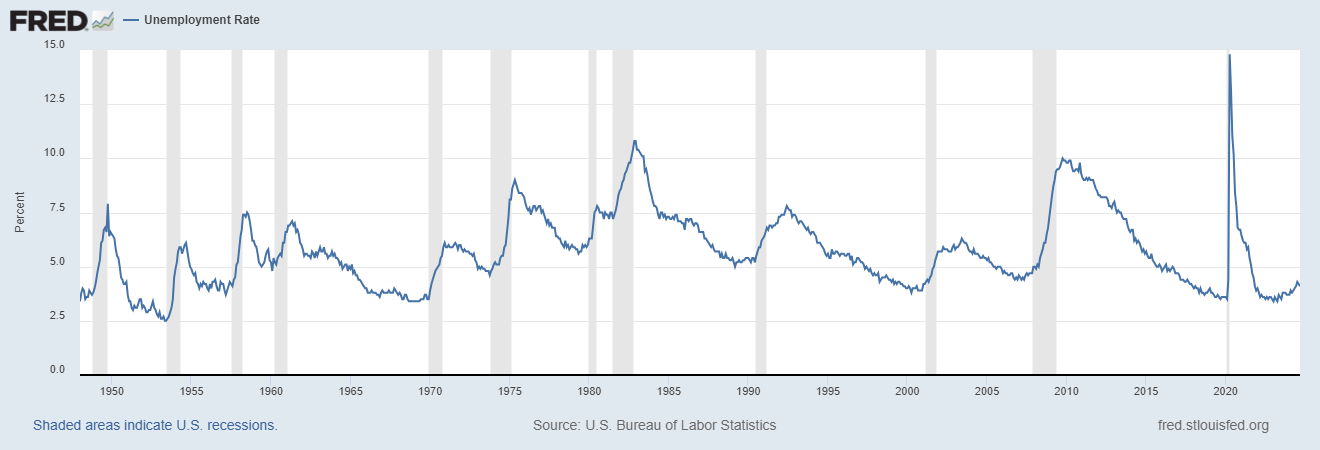
\includegraphics[width=0.65\linewidth]{figs/FREDBC.png}
\end{figure}
\item <+->Rest of the course:
\begin{itemize}
\item Study how aggregate shocks cause business cycles
\begin{itemize}
\item Does the transmission change with heterogeneous agents?
\end{itemize}
\item Implications for fiscal and monetary policy
\end{itemize}
\end{itemize}
\end{frame}
%

\section{IS-LM}

\begin{frame}{The IS-LM model}
\begin{itemize}
  \item Aggregate demand is $D=C+G$ (abstracting away from investment) \pause
  \item Assume $C=c_0+c_1(Y-T)-c_2r$ with $c_1\in(0,1)$  \pause
  \item If output is demand determined, then $Y=D$, and $$Y = \frac{1}{1-c_1}(c_0 - c_1 T + G - c_2 r)$$ \pause
  \item \textbf{Core intuition}: \underline{all of income is somebody else's spending!}
\end{itemize}
\end{frame}
%
\begin{frame}{Block representation}
\begin{center}
\begin{tikzpicture}[blk/.style={draw,rounded corners=2pt,minimum width=26mm,minimum height=9mm,align=center,font=\small},var/.style={font=\small},lab/.style={font=\small,inner sep=1.5pt},>=stealth]
\node[var] (in) at (-0.6,0) {Policy};
\node[blk,fill=DarkRed!15] (c) at (3.2,0) {Consumption\\$C(Y-T,r)$};
\node[blk] (mc) at (7,0) {Goods market\\$Y=C+G$};
\node[var] (y) at (9.8,0) {Output};
\draw[->] (in)--node[lab,above]{$T,r$}(c);
\draw[->] (c)--node[lab,above]{$C$}(mc);
\draw[->] (mc)--node[lab,above]{$Y$}(y);
\draw[->] (y.north) |- (5.1,1.1) node[lab,above]{$Y$} -| (c.north);
\draw[->] (in.south) |- (7,-1.1) node[lab,pos=0.75,below]{$G$} -- (mc.south);
\end{tikzpicture}
\end{center}
\begin{itemize}
\item <+->Consumption is the only behavioral block
\item <+->Output feeds back into consumption through income
\item <+->We keep this structure for the whole lecture
\end{itemize}
\end{frame}
%
\begin{frame}{Policies in IS-LM}
\begin{itemize}
  \item \textbf{Fiscal policy:} multiplier is $\frac{dY}{dG}=\frac{1}{1-c_1}>1$ \pause
  \item \textbf{Monetary policy:} multiplier is $\frac{dY}{dr}=-\frac{c_2}{1-c_1}<0$ \pause
  \begin{itemize}
    \item Direct effect is $-c_2$  \pause
    \item Indirect effect through $Y$ is $c_1 \frac{dY}{dr}$ \pause
  \end{itemize}
  \item What's missing? \pause
  \begin{itemize}
    \item A supply side, micro-foundations, expectations, etc.
  \end{itemize}
\end{itemize}
\end{frame}
%
\begin{frame}{Can we get this in a micro-founded model?}
\begin{itemize}
\item <+->\textbf{IS-LM:} $G$ raises demand, output rises, income rises, demand rises further: a multiplier above 1
\item <+->But no budget constraints and no expectations
\item <+->In HANK we can get this back, with \textbf{two ingredients}:
\begin{enumerate}
\item \textbf{Nominal rigidities:} output is demand determined
\item \textbf{Departure from Ricardian equivalence:} the timing of income moves spending
\end{enumerate}
\end{itemize}

\end{frame}
%

\section{NK framework}

\begin{frame}{New Keynesian framework}
\begin{itemize}
\item <+-> A proper model of business cycles and stabilization policy requires
that output is partially demand determined
\item <+-> The study of monetary policy requires \textbf{monetary non-neutrality}
\item <+-> The New Keynesian (NK) model addresses these two concerns by
adding to the standard model:
\begin{itemize}
\item Monopolistic competition (wage-setting by unions)
\item Wage rigidities
\end{itemize}
\item <+->Textbooks use sticky prices. We use sticky wages, and the reason comes at the end of the lecture
\end{itemize}
\end{frame}
%
\begin{frame}{The model}
The model consists of the following agents:
\begin{itemize}
\item[1.] \textbf{Households} who consume and save
\item[2.] \textbf{Firms} with market power who produce using labor and set prices
\item[3.] \textbf{Unions} with market power who set wages subject to nominal rigidities
\item[4.] A \textbf{mutual fund} which holds stocks and bonds
\item[5.] A \textbf{government} that spends, taxes and issues nominal bonds
\item[6.] A \textbf{central bank} which follows a Taylor rule
\end{itemize}

\textit{Note:} We leave the household problem open for now

\end{frame}

%
\begin{frame}{Block representation}
\blockdag{Households}{$C^{hh}(\boldsymbol{Z},\boldsymbol{r}^{p})$}
\begin{itemize}
\item <+->\textbf{Read it left to right:} guess $\boldsymbol{\pi}^{w},\boldsymbol{L}$, compute the aggregate blocks, get consumption, check the two targets
\item <+->$Z_{t}$ is post-tax labor income
\item <+->The red box is left open: RANK, TANK and HANK fill it in, nothing else changes
\end{itemize}
\end{frame}
%
\begin{frame}{Firms}
\begin{itemize}
\item <+->\textbf{Production:} $Y_{t}=L_{t}$
\item <+->\textbf{Prices:} firms set a constant markup $\mu$ over marginal cost, prices are flexible:
\[
P_{t}=\mu W_{t}\quad\Rightarrow\quad w_{t}\equiv\frac{W_{t}}{P_{t}}=\frac{1}{\mu}
\]
\item <+->So \textbf{price inflation equals wage inflation:} $\pi_{t}=\pi_{t}^{w}$
\item <+->\textbf{Dividends}, taxed at the same rate as labor income:
\[
d_{t}=(1-\tau_{t})\left(Y_{t}-\frac{L_{t}}{\mu}\right)=(1-\tau_{t})\left(1-\frac{1}{\mu}\right)Y_{t}
\]
\end{itemize}
\end{frame}
%
\begin{frame}{Unions}
\begin{itemize}
\item <+->Unions indexed by $j\in[0,1]$ each supply a differentiated labor type (Erceg, Henderson and Levin, 2000)
\item <+->Firms use a CES bundle of labor types with sub. elasticity $\epsilon^{W}$, so \textbf{labor demand} for union $j$ is
\[
L_{t}^{j}=\left(\frac{W_{t}^{j}}{W_{t}}\right)^{-\epsilon^{W}}L_{t}
\]
\item <+->Union $j$ sets its wage $W_{t}^{j}$ and supplies what firms demand
\item <+->Changing wages has a quadratic \emph{utility} cost $\Rightarrow$ sticky wages
\item <+->\textbf{Note:} no resource cost, so goods market clearing is unchanged
\end{itemize}
\end{frame}
%
\begin{frame}{Union problem}
\begin{itemize}
\item <+->\textbf{Bellman equation of the union:} the state is last period's wage
\begin{align*}
V_{t}\left(W_{t-1}^{j}\right)=\max_{W_{t}^{j}} & \left\{ u'\left(C_{t}\right)(1-\tau_{t})\frac{W_{t}^{j}}{P_{t}}L_{t}^{j}-h\left(L_{t}^{j}\right)\right.\\
 & \left.-\frac{\theta^{W}}{2}\left(\frac{W_{t}^{j}}{W_{t-1}^{j}}-1\right)^{2}+\beta E_{t}V_{t+1}\left(W_{t}^{j}\right)\right\}
\end{align*}
subject to labor demand
\item <+->\textbf{FOC wrt. $W_{t}^{j}$}, using labor demand:
\begin{align*}
0= & \left(1-\epsilon^{W}\right)(1-\tau_{t})u'\left(C_{t}\right)\frac{L_{t}^{j}}{P_{t}}+\epsilon^{W}h'\left(L_{t}^{j}\right)\frac{L_{t}^{j}}{W_{t}^{j}}\\
 & -\frac{\theta^{W}}{W_{t-1}^{j}}\left(\frac{W_{t}^{j}}{W_{t-1}^{j}}-1\right)+\beta E_{t}V_{t+1}^{\prime}\left(W_{t}^{j}\right)
\end{align*}
\item <+->\textbf{Envelope condition:} $V_{t}^{\prime}\left(W_{t-1}^{j}\right)=\theta^{W}\left(\frac{W_{t}^{j}}{W_{t-1}^{j}}-1\right)\frac{W_{t}^{j}}{\left(W_{t-1}^{j}\right)^{2}}$
\end{itemize}
\end{frame}
%
\begin{frame}{Derivation of W-NKPC}
\begin{itemize}
\item <+->\textbf{Symmetry:} all unions set the same wage, $W_{t}^{j}=W_{t}$, $L_{t}^{j}=L_{t}$
\item <+->Multiply the FOC by $W_{t}/\theta^{W}$, with $W_{t}/P_{t}=1/\mu$:
\[
\pi_{t}^{w}\left(1+\pi_{t}^{w}\right)=\kappa\left\{ h'\left(L_{t}\right)-\frac{1-\tau_{t}}{\mu\mu^{w}}u'\left(C_{t}\right)\right\} L_{t}+\beta E_{t}\pi_{t+1}^{w}\left(1+\pi_{t+1}^{w}\right)
\]
with slope $\kappa=\frac{\epsilon^{W}}{\theta^{W}}$ and wage markup $\mu^{w}=\frac{\epsilon^{W}}{\epsilon^{W}-1}$
\item <+->\textbf{Simpler version} with the same first-order approximation around $\pi^{w}=0$, $L=1$:
\[
\pi_{t}^{w}=\kappa\left(h'\left(L_{t}\right)-\frac{1-\tau_{t}}{\mu\mu^{w}}u'\left(C_{t}\right)\right)+\beta E_{t}\pi_{t+1}^{w}
\]
\end{itemize}
\end{frame}
%
\begin{frame}{What sticky wages mean}
\begin{itemize}
\item <+->Nominal wages $W_{t}$ adjust only partly, slowly through the W-NKPC
\item <+->At this wage, unions supply whatever labor firms ask for
\item <+->Firms produce what is demanded and hire $L_{t}=Y_{t}$
\item <+->So \textbf{output is demand determined}: demand sets $Y_{t}$, and $Y_{t}$ sets $L_{t}$
\item <+->Households are off their labor supply curve in the short run
\item <+->Over time, unions raise wages if $L_{t}$ is high: that is the W-NKPC
\item <+->Because of flexible prices, full path through to goods inflation: $\pi_t=\pi_t^w$
\end{itemize}
\end{frame}

%
\begin{frame}{Fiscal authority}
\begin{itemize}
\item <+->\textbf{Budget:} spending $G_{t}$, taxes $T_{t}$, nominal debt with real value $B_{t}$
\[
T_{t}=(1+r_{t}^{b})B_{t-1}+G_{t}-B_{t},\quad T_{t}=\tau_{t}Y_{t},\quad1+r_{t}^{b}=\frac{1+i_{t-1}}{1+\pi_{t}}
\]
\item <+->The government chooses the paths of $G_{t}$ and $B_{t}$, with $B_{t}\rightarrow B_{ss}$
\item <+->Taxes adjust to satisfy the budget
\item <+->\textbf{Deficit:} with a constant return on debt, and $\boldsymbol{L}$ the lag matrix, it only depends on the debt path:
\[
d\boldsymbol{G}-d\boldsymbol{T}=\left(\boldsymbol{I}-(1+r_{ss})\boldsymbol{L}\right)d\boldsymbol{B}
\]
\item <+->Debt returns to steady state, so with $q_{t}=(1+r_{ss})^{-t}$ the deficit has zero present value: $\boldsymbol{q}^{\prime}(d\boldsymbol{G}-d\boldsymbol{T})=0$
\item <+->\textbf{Balanced budget:} $B_{t}=B_{ss}$
\item <+->\textbf{Deficit financing:} debt rises first, and taxes repay it later
\end{itemize}
\end{frame}
%
\begin{frame}{Central bank}
\begin{itemize}
\item <+->\textbf{Monetary policy} follows a Taylor rule:
\[
i_{t}=i_{ss}+\phi\pi_{t}
\]
\item <+->\textbf{Fisher relationship} links the nominal and the real rate:
\[
1+r_{t}=\frac{1+i_{t}}{1+\pi_{t+1}}
\]
\item <+->Monetary policy matters because wages are sticky: inflation does not move 1-1 with $i_{t}$, so $r_{t}$ moves
\end{itemize}
\end{frame}
%
\begin{frame}{Mutual fund}
\vspace{-1mm}
\begin{itemize}
\item <+->Collects household savings and holds stocks and bonds: $A_{t}=p_{t}+B_{t}$
\item <+->A mass 1 of shares with price $p_{t}$. No arbitrage with bonds:
\[
\underset{\text{real bonds}}{\underbrace{1+r_{t}}}=\underset{\text{return on equity}}{\underbrace{\frac{p_{t+1}+d_{t+1}}{p_{t}}}}=\underset{\text{nominal bonds}}{\underbrace{\frac{1+i_{t}}{1+\pi_{t+1}}}}
\]
\item <+->\textbf{Return from $t=1$ on:} known in advance, so $r_{t+1}^{p}=r_{t}$
\item <+->\textbf{Return at $t=0$:} a surprise shock revalues the portfolio
\[
1+r_{0}^{p}=\underset{\text{capital gains}}{\underbrace{\frac{p_{0}+d_{0}}{A_{ss}}}}+\underset{\text{inflation revaluation}}{\underbrace{\frac{1+i_{ss}}{1+\pi_{0}}\frac{B_{ss}}{A_{ss}}}}
\]
\item <+->\textbf{Inflation:} bonds pay the nominal rate $i_{ss}$ set before the shock. If $\pi_{0}$ rises, their real value falls, and so does $r_{0}^{p}$
\item <+->\textbf{Stocks:} if expected dividends rise or $r$ falls, $p_{0}$ rises, and so does $r_{0}^{p}$
\end{itemize}
\end{frame}
%
\begin{frame}{Households}
\begin{itemize}
\item <+->Households save in the mutual fund and take income and returns as given:
\[
C_{t}+A_{t}=\left(1+r_{t}^{p}\right)A_{t-1}+Z_{t},\quad Z_{t}=\frac{1-\tau_{t}}{\mu}L_{t}^{hh}
\]
\item <+->Labor supply $L_{t}^{hh}$ is set by the union
\item <+->We leave the household problem open for now. All we need is an \textbf{aggregate consumption function:}
\[
\boldsymbol{C}^{hh}=C^{hh}\left(\boldsymbol{Z},\boldsymbol{r}^{p}\right)
\]
\item <+->Consumption depends on the whole path of income and of $r_{t}^{p}$, the return on the mutual fund. Households do not care about $r_{t}$ or $i_{t}$ directly
\end{itemize}
\end{frame}
%
\begin{frame}{Equilibrium}
\begin{itemize}
\item <+->Three markets:
\[
Y_{t}=C_{t}+G_{t},\quad L_{t}^{hh}=L_{t},\quad A_{t}=p_{t}+B_{t}
\]
\item <+->By Walras' law, we can drop one of them: the diagram targets goods, the HANK code targets assets
\item <+->\textbf{Goods market} has the same structure as IS-LM:
\[
\boldsymbol{Y}=\boldsymbol{G}+C^{hh}(\boldsymbol{Z},\boldsymbol{r}^{p})
\]
\item <+->\textbf{Supply side:} the W-NKPC, with feedback through the Taylor rule
\item <+->In general, solving this requires a computer
\end{itemize}
\end{frame}
%
\begin{frame}{Equations summary}
\vspace{-3mm}
{\footnotesize
\begin{align*}
\text{Households:}\quad & \boldsymbol{C}=C^{hh}(\boldsymbol{Z},\boldsymbol{r}^{p}),\quad C_{t}+A_{t}=(1+r_{t}^{p})A_{t-1}+Z_{t}\\
 & Z_{t}=\frac{1-\tau_{t}}{\mu}L_{t}\\
\text{Firms:}\quad & Y_{t}=L_{t},\quad\pi_{t}=\pi_{t}^{w},\quad d_{t}=(1-\tau_{t})\left(1-\frac{1}{\mu}\right)Y_{t}\\
\text{Union:}\quad & \pi_{t}^{w}=\kappa\left(h'\left(L_{t}\right)-\frac{1-\tau_{t}}{\mu\mu^{w}}u'\left(C_{t}\right)\right)+\beta\pi_{t+1}^{w}\\
\text{Mutual fund:}\quad & A_{t}=p_{t}+B_{t},\quad1+r_{t}=\frac{p_{t+1}+d_{t+1}}{p_{t}}=\frac{1+i_{t}}{1+\pi_{t+1}},\quad r_{t+1}^{p}=r_{t}\\
\text{Government:}\quad & T_{t}=(1+r_{t}^{b})B_{t-1}+G_{t}-B_{t},\quad T_{t}=\tau_{t}Y_{t}\\
\text{Central bank:}\quad & i_{t}=i_{ss}+\phi\pi_{t}\\
\text{Market clearing:}\quad & Y_{t}=C_{t}+G_{t}
\end{align*}
}
\begin{itemize}
\item <+->Exogenous: $G_{t}$ and $B_{t}$
\item <+->$C^{hh}$ is the only equation that changes across RANK, TANK and HANK
\end{itemize}
\end{frame}
%
\begin{frame}{Experiments and calibration}
\begin{itemize}
\item <+->\textbf{Frequency:} annual, with $r_{ss}=2\%$, $G_{ss}=20\%$ of output and $\kappa=0.16$
\item <+->\textbf{Shock:} a surprise at $t=0$ (an ``MIT shock''). After that, there is no uncertainty, so agents know the whole future path: perfect foresight
\item <+->\textbf{Spending:} $dG_{t}=\rho_{G}dG_{t-1}$, with $dG_{0}=1\%$ of output and $\rho_{G}=0.8^{4}\approx0.41$
\item <+->\textbf{Debt:} $dB_{t}=\rho_{B}\left(dB_{t-1}+dG_{t}\right)$. $\rho_{B}=0$ is a balanced budget, and the baseline is $\rho_{B}=0.9$
\item <+->We solve the model to first order in the sequence space, as in lectures 5-6
\end{itemize}
\end{frame}
%

\section{Deriving the IKC for a fiscal shock}

\begin{frame}{Three assumptions}
\begin{itemize}
\item <+->To get analytical results, we make three assumptions
\begin{enumerate}
    \item <+->\textbf{Real rate rule:} $1+i_{t}=(1+r_{ss})(1+\pi_{t+1})$, so $r_{t}=r_{ss}$
    \begin{itemize}
        \item A Taylor rule with a coefficient of 1 on expected inflation
        \item A middle ground between loose policy (ZLB) and tight policy (active Taylor rule)
    \end{itemize}
    \item <+->\textbf{Real bonds:} no revaluation of debt from surprise inflation at $t=0$
    \item <+->\textbf{No markups:} $\mu=1$, so $d_{t}=0$, $p_{t}=0$ and $A_{t}=B_{t}$
\end{enumerate}

\item <+->Together: $r_{t}^{p}=r_{ss}$ at all dates, so $C^{hh}(\boldsymbol{Z},\boldsymbol{r}^{p})$ becomes $C^{hh}(\boldsymbol{Z})$
\item <+->Inflation is irrelevant to output
\end{itemize}

\end{frame}
%
\begin{frame}{Simplified system of equations}
\vspace{-2mm}
{\small
\begin{align*}
\text{Households:}\quad & \boldsymbol{C}=C^{hh}(\boldsymbol{Z}),\quad C_{t}+A_{t}=(1+r_{ss})A_{t-1}+Z_{t},\quad Z_{t}=Y_{t}-T_{t}\\
\text{Firms:}\quad & Y_{t}= L_{t} \\
\text{Government:}\quad & T_{t}=(1+r_{ss})B_{t-1}+G_{t}-B_{t},\quad T_{t}=\tau_{t}Y_{t}\\
\text{Market clearing:}\quad & Y_{t}=C_{t}+G_{t},\quad A_{t}=B_{t}
\end{align*}
}
\begin{itemize}
\item <+->The debt path and the government budget give $\boldsymbol{T}$
\item <+->Goods market clearing alone then gives $\boldsymbol{Y}$:
\[
\boldsymbol{Y}=\boldsymbol{G}+C^{hh}(\boldsymbol{Y}-\boldsymbol{T})
\]
\item <+->The W-NKPC still gives inflation, and the central bank gives $i_{t}$, but they are not needed to determine $Y$
\end{itemize}
\end{frame}
%
\begin{frame}{Block representation of the IKC model}
\ikcdag{Households}{$C^{hh}(\boldsymbol{Z})$}
\begin{itemize}
\item <+->One unknown, one target: $r$ is fixed, and firms and the fund play no role
\item <+->Taxes depend only on the shocks, not on $\boldsymbol{Y}$
\end{itemize}
\end{frame}
%
\begin{frame}{Why $C(\boldsymbol{Z})$ and not $C(\boldsymbol{Y},\boldsymbol{T})$?}
\begin{itemize}
\item <+->\textbf{Income:} with $\mu=1$, $d_{t}=0$, so all of $Y_{t}$ is labor income
\item <+->\textbf{Taxes:} $T_{t}=\tau_{t}Y_{t}$ hit that same income in proportion:
\[
Z_{t}=(1-\tau_{t})Y_{t}=Y_{t}-T_{t}
\]
\item <+->Households only see the difference: one more unit of output and one less unit of taxes have the same effect
\item <+->So one matrix is enough, and it applies to $d\boldsymbol{Y}-d\boldsymbol{T}$
\end{itemize}
\end{frame}
%
\begin{frame}{Aggregate consumption function in the sequence space}
\begin{itemize}
\item <+->Households are forward-looking, and the whole path of income is known at $t=0$
\item <+->So consumption at date $t$ depends on income at \emph{all} dates, not just on $Z_{t}$:
\[
C_{t}^{hh}=C_{t}^{hh}\left(Z_{0},Z_{1},Z_{2},\dots\right)\quad\text{for all }t
\]
Stacking all dates gives the vector function $\boldsymbol{C}^{hh}=C^{hh}(\boldsymbol{Z})$
\item <+->\textbf{Total differentiation} around steady state:
\[
dC_{t}^{hh}=\sum_{s=0}^{\infty}\frac{\partial C_{t}^{hh}}{\partial Z_{s}}dZ_{s}
\]
\item <+->In vector form, with $\boldsymbol{M}$ the \textbf{matrix of intertemporal MPCs (iMPCs)}:
\[
d\boldsymbol{C}^{hh}=\boldsymbol{M}d\boldsymbol{Z},\quad M_{t,s}=\frac{\partial C_{t}^{hh}}{\partial Z_{s}}
\]
\item <+->$M_{t,s}$: how much $C_{t}$ moves when $Z_{s}$ moves. $\boldsymbol{M}$ encodes the entire \emph{complexity of HH behavior}
\end{itemize}
\end{frame}
%
\begin{frame}{The iMPC matrix $\boldsymbol{M}$}
\vspace{-1mm}
\begin{center}
\begin{tikzpicture}[lab/.style={font=\small},ampersand replacement=\&]
\matrix (M) [matrix of math nodes,left delimiter={[},right delimiter={]},nodes={minimum width=17mm,minimum height=7mm,anchor=center}] {
M_{0,0} \& M_{0,1} \& M_{0,2} \& \cdots\\
M_{1,0} \& M_{1,1} \& M_{1,2} \& \cdots\\
M_{2,0} \& M_{2,1} \& M_{2,2} \& \cdots\\
\vdots \& \vdots \& \vdots \& \ddots\\
};
\node[lab] at (M-1-1.north |- 0,1.75) {$s=0$};
\node[lab] at (M-1-2.north |- 0,1.75) {$s=1$};
\node[lab] at (M-1-3.north |- 0,1.75) {$s=2$};
\node[lab,anchor=east] at (-4.5,0 |- M-1-1) {$t=0$};
\node[lab,anchor=east] at (-4.5,0 |- M-2-1) {$t=1$};
\node[lab,anchor=east] at (-4.5,0 |- M-3-1) {$t=2$};
\begin{scope}[on background layer]
\onslide<2->{\node[fill=DarkRed!20,draw=DarkRed,rounded corners=3pt,fit=(M-1-2)(M-4-2),inner sep=0pt] {};}
\onslide<4->{\node[fill=blue!15,draw=blue!60!black,rounded corners=3pt,fit=(M-3-1)(M-3-4),inner sep=0pt,fill opacity=0.6] {};}
\end{scope}
\end{tikzpicture}
\end{center}
\begin{itemize}
\item<2-> \textcolor{DarkRed}{\textbf{Column $s$:}} the path of consumption after one more unit of income at date $s$. Each column is an impulse response
\item<3-> For $s>0$, households learn at $t=0$ that income rises at $s$, so they can react before it arrives
\item<4-> \textcolor{blue!60!black}{\textbf{Row $t$:}} how much consumption at date $t$ reacts to income at each date
\item<5-> $M_{0,0}$ is essentially the annual MPC
\end{itemize}
\end{frame}
%
\begin{frame}{Intertemporal Keynesian Cross}
\begin{itemize}
\item <+->Combine goods market clearing and the consumption function:
\[
\boldsymbol{Y}=\boldsymbol{G}+C^{hh}(\boldsymbol{Y}-\boldsymbol{T})
\]
\item <+->Differentiate, using $d\boldsymbol{C}^{hh}=\boldsymbol{M}d\boldsymbol{Z}$ and $d\boldsymbol{Z}=d\boldsymbol{Y}-d\boldsymbol{T}$. This is the \textbf{Intertemporal Keynesian Cross}:
\begin{align*}
d\boldsymbol{Y} & =d\boldsymbol{G}+\boldsymbol{M}\left(d\boldsymbol{Y}-d\boldsymbol{T}\right)\Leftrightarrow\\
(\boldsymbol{I}-\boldsymbol{M})d\boldsymbol{Y} & =d\boldsymbol{G}-\boldsymbol{M}d\boldsymbol{T}
\end{align*}
\item <+->The whole model reduces to one equation, and $\boldsymbol{M}$ is a sufficient statistic: same iMPCs imply the same $d\boldsymbol{Y}$
\end{itemize}
\end{frame}
%
\begin{frame}{Balanced budget multiplier}
\begin{itemize}
\item <+->\textbf{Balanced budget:} debt does not move, $d\boldsymbol{B}=\boldsymbol{0}$, so $d\boldsymbol{T}=d\boldsymbol{G}$
\item <+->The IKC becomes
\[
d\boldsymbol{Y}=d\boldsymbol{G}+\boldsymbol{M}\left(d\boldsymbol{Y}-d\boldsymbol{G}\right)\quad\Leftrightarrow\quad(\boldsymbol{I}-\boldsymbol{M})\left(d\boldsymbol{Y}-d\boldsymbol{G}\right)=\boldsymbol{0}
\]
\item <+->So $d\boldsymbol{Y}=d\boldsymbol{G}$ solves it, for \textbf{any} $\boldsymbol{M}$
\item <+->\textbf{Intuition:} output rises by $dG_{t}$ and taxes by $dG_{t}$, so post-tax income does not change, and neither does consumption: $d\boldsymbol{C}=\boldsymbol{0}$
\item <+->Multiplier of exactly 1, whatever the household block: RANK, TANK or HANK
\item <+->So the household block only matters for deficits
\end{itemize}
\end{frame}
%
\begin{frame}{Illustration}
\begin{itemize}
\item Writing out the IKC:
\[
\begin{aligned}\begin{bmatrix}dY_{0}\\
dY_{1}\\
dY_{2}\\
\vdots
\end{bmatrix} & =\begin{bmatrix}dG_{0}\\
dG_{1}\\
dG_{2}\\
\vdots
\end{bmatrix}+\begin{bmatrix}\frac{\partial C_{0}^{hh}}{\partial Z_{0}} & \frac{\partial C_{0}^{hh}}{\partial Z_{1}} & \frac{\partial C_{0}^{hh}}{\partial Z_{2}} & \cdots\\
\frac{\partial C_{1}^{hh}}{\partial Z_{0}} & \frac{\partial C_{1}^{hh}}{\partial Z_{1}} & \frac{\partial C_{1}^{hh}}{\partial Z_{2}} & \cdots\\
\frac{\partial C_{2}^{hh}}{\partial Z_{0}} & \frac{\partial C_{2}^{hh}}{\partial Z_{1}} & \frac{\partial C_{2}^{hh}}{\partial Z_{2}} & \cdots\\
\vdots & \vdots & \vdots & \ddots
\end{bmatrix}\left(\begin{bmatrix}dY_{0}\\
dY_{1}\\
dY_{2}\\
\vdots
\end{bmatrix}-\begin{bmatrix}dT_{0}\\
dT_{1}\\
dT_{2}\\
\vdots
\end{bmatrix}\right)\end{aligned}
\]
\end{itemize}
\end{frame}
%
\begin{frame}{Tricky point: inverting $\boldsymbol{I}-\boldsymbol{M}$}
\begin{itemize}
\item <+->\textbf{Issue:} we cannot solve the IKC by inverting $\boldsymbol{I}-\boldsymbol{M}$. In every model with a budget constraint, households eventually spend every unit of income, so
\[
\boldsymbol{q}^{\prime}(\boldsymbol{I}-\boldsymbol{M})=\boldsymbol{0}\quad\text{(proof on the next slide)}
\]
\item <+->\textbf{One equation is redundant:} multiply the IKC by $\boldsymbol{q}^{\prime}$
\[
\underset{=0}{\underbrace{\boldsymbol{q}^{\prime}(\boldsymbol{I}-\boldsymbol{M})d\boldsymbol{Y}}}=\boldsymbol{q}^{\prime}(d\boldsymbol{G}-\boldsymbol{M}d\boldsymbol{T})=\boldsymbol{q}^{\prime}(d\boldsymbol{G}-d\boldsymbol{T})
\]
This is just the government budget: it holds for any $d\boldsymbol{Y}$
\item <+->\textbf{Many solutions:} in RANK, $\boldsymbol{M}^{RA}\boldsymbol{1}=\boldsymbol{1}$, so a permanent rise in $d\boldsymbol{Y}$ can be added to any solution
\item <+->We pick the one where $d\boldsymbol{Y}$ returns to zero:
\[
d\boldsymbol{Y}=\mathcal{M}(d\boldsymbol{G}-\boldsymbol{M}d\boldsymbol{T}),\quad\mathcal{M}:\text{ inverse of }\boldsymbol{I}-\boldsymbol{M}\text{ on paths that return to zero}
\]
\item <+->\textbf{Numerically:} truncation at a finite horizon makes $\boldsymbol{I}-\boldsymbol{M}$ invertible, but precision worsens with the horizon
\end{itemize}
\end{frame}
%
\begin{frame}{Tricky point: proof}
\vspace{-1mm}
\begin{itemize}
\item <+->\textbf{Step 1:} linearize the household budget, with $dA_{-1}=0$ and constant $r$:
\[
dC_{t}+dA_{t}=(1+r_{ss})dA_{t-1}+dZ_{t}
\]
\item <+->\textbf{Step 2:} multiply by $q_{t}=(1+r_{ss})^{-t}$ and sum over $t$. Since $q_{t}(1+r_{ss})=q_{t-1}$, the asset terms cancel out:
\[
\sum_{t=0}^{T}q_{t}dC_{t}+q_{T}dA_{T}=\sum_{t=0}^{T}q_{t}dZ_{t}
\]
\item <+->\textbf{Step 3:} let $T\rightarrow\infty$, with assets back at steady state, $dA_{T}\rightarrow0$:
\[
\boldsymbol{q}^{\prime}d\boldsymbol{C}^{hh}=\boldsymbol{q}^{\prime}d\boldsymbol{Z}
\]
\item <+->\textbf{Step 4:} use $d\boldsymbol{C}^{hh}=\boldsymbol{M}d\boldsymbol{Z}$. This holds for any $d\boldsymbol{Z}$, so
\[
\boldsymbol{q}^{\prime}\boldsymbol{M}=\boldsymbol{q}^{\prime}\quad\Leftrightarrow\quad\boldsymbol{q}^{\prime}(\boldsymbol{I}-\boldsymbol{M})=\boldsymbol{0}
\]
\item <+->So no inverse: if $(\boldsymbol{I}-\boldsymbol{M})^{-1}$ existed, multiplying by it would give $\boldsymbol{q}^{\prime}=\boldsymbol{0}$
\end{itemize}
\end{frame}
%
\begin{frame}{Solving the IKC}
\vspace{-2mm}
\begin{itemize}
\item <+->Rewrite the IKC in terms of consumption:
\begin{align*}
d\boldsymbol{Y}-d\boldsymbol{G} & =\boldsymbol{M}(d\boldsymbol{G}-d\boldsymbol{T})+\boldsymbol{M}(d\boldsymbol{Y}-d\boldsymbol{G})\\
\Rightarrow d\boldsymbol{Y} & =d\boldsymbol{G}+\underset{d\boldsymbol{C}}{\underbrace{\mathcal{M}\boldsymbol{M}(d\boldsymbol{G}-d\boldsymbol{T})}}
\end{align*}
\item <+->$d\boldsymbol{T}$ is exogenous: $dT_{t}=dG_{t}+(1+r_{ss})dB_{t-1}-dB_{t}$. The tax rate $\tau_{t}=T_{t}/Y_{t}$ adjusts
\item <+->\textbf{Deficits:} $d\boldsymbol{G}\neq d\boldsymbol{T}$
\begin{itemize}
\item All the action in $d\boldsymbol{C}$ comes from the deficit
\item This is where the household block matters
\end{itemize}
\end{itemize}
\end{frame}
%
\begin{frame}{Fiscal multipliers}

\textbf{Impact multiplier:}
\[
\frac{\partial Y_{0}}{\partial G_{0}}
\]
\textbf{Cumulative multiplier:}
\[
\frac{\sum_{t=0}^{\infty}(1+r_{ss})^{-t}dY_{t}}{\sum_{t=0}^{\infty}(1+r_{ss})^{-t}dG_{t}}=\frac{\boldsymbol{q}^{\prime}d\boldsymbol{Y}}{\boldsymbol{q}^{\prime}d\boldsymbol{G}}
\]

\end{frame}
%
\begin{frame}{What do we know about $\boldsymbol{M}$?}
\begin{itemize}
\item <+->If we knew all of $\boldsymbol{M}$ from the data, we would not need a model: the IKC gives $d\boldsymbol{Y}$
\item <+->We only observe the first column: Fagereng et al., lottery winnings\\
\begin{figure}[H]
\centering
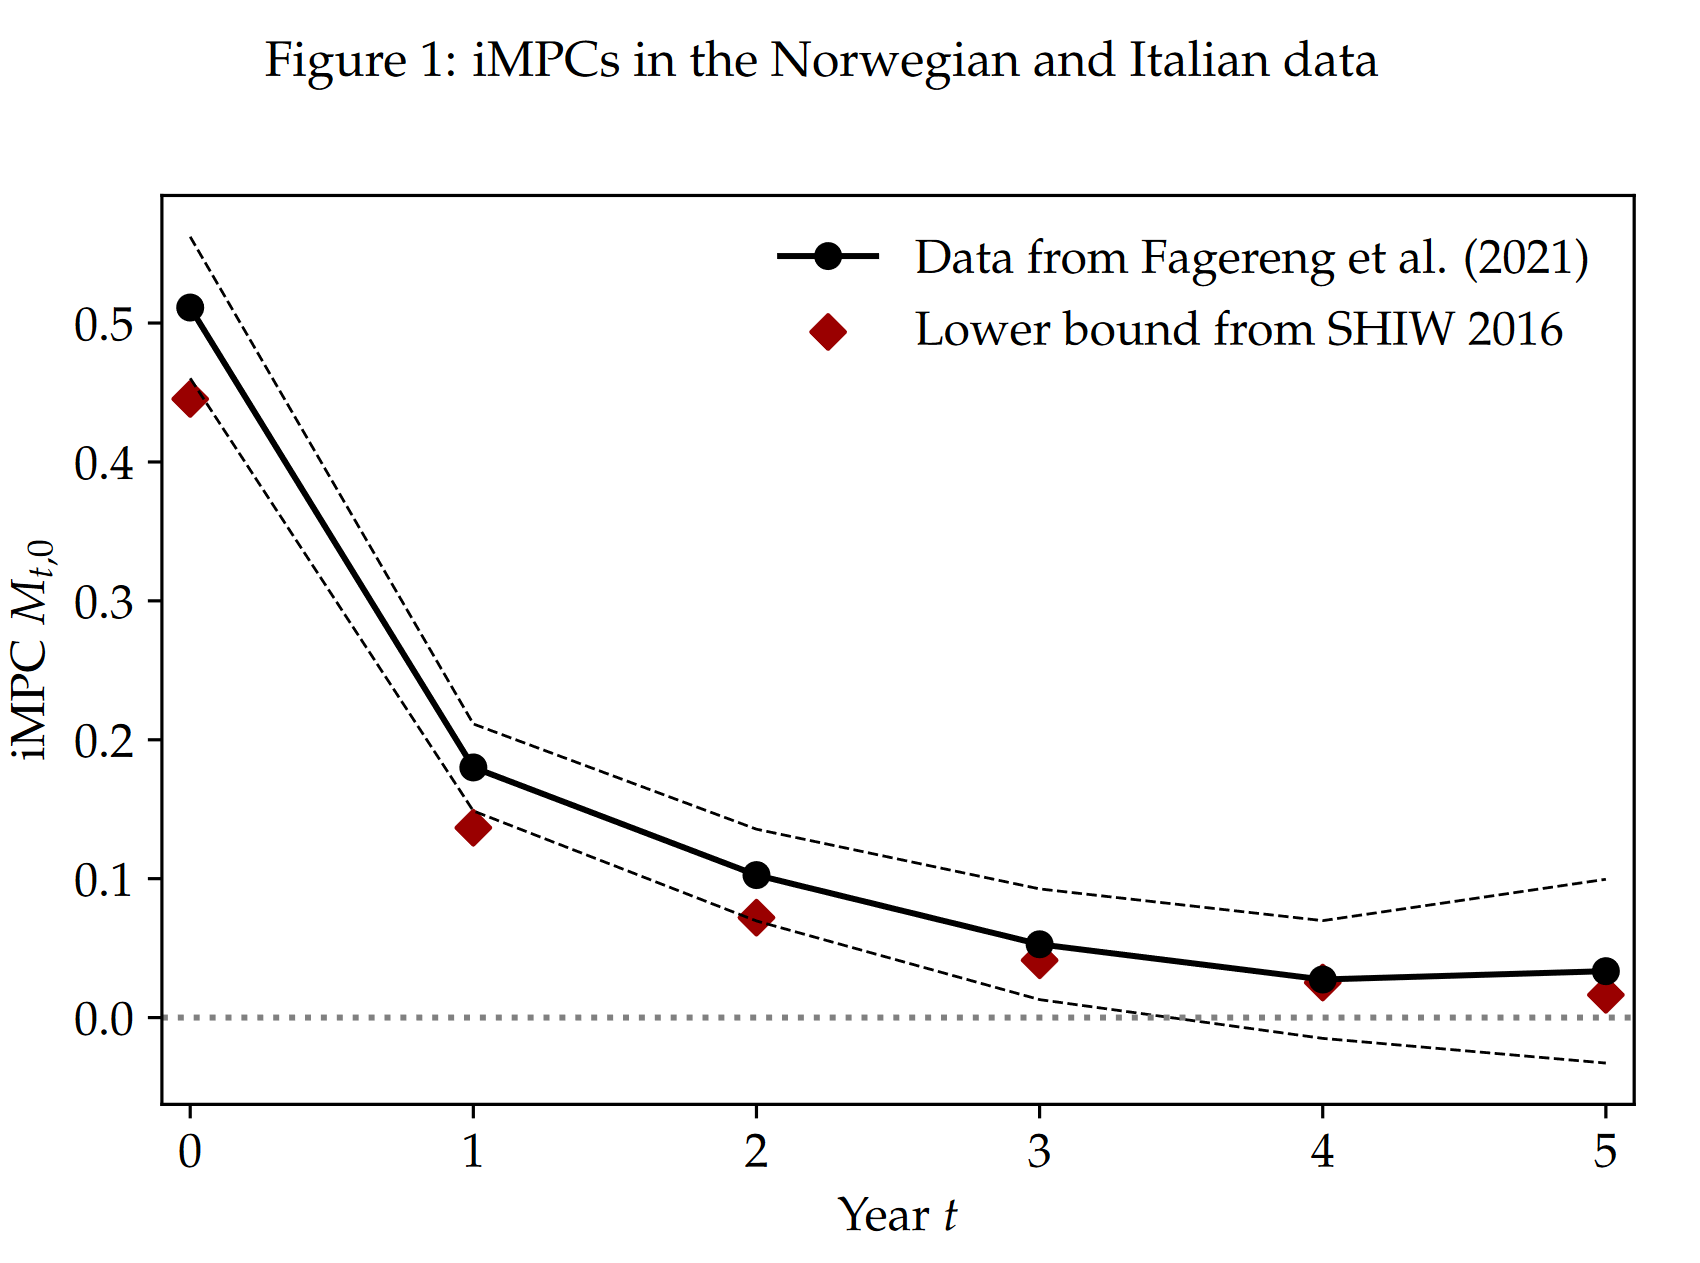
\includegraphics[width=0.46\linewidth]{figs/iMPC_data.png}
\end{figure}
\item <+->Annual MPC above 0.5, then 0.18 the year after
\item <+->{\footnotesize{}Other columns (announcements) are very hard to estimate. So we need models: RANK, TANK and HANK are different microfoundations of $\boldsymbol{M}$}{\footnotesize\par}
\end{itemize}
\end{frame}
%
\begin{frame}{Rest of the course: different models of $\boldsymbol{M}$}
\begin{itemize}
\item RANK, TANK and HANK are different microfoundations of $C^{hh}$, and so of $\boldsymbol{M}$
\item Spoiler for the rest of the class:
\end{itemize}
\vspace{2mm}
\begin{center}
\begin{tabular}{lccc}
 & \textbf{Ricardian equivalence} & \textbf{Impact} & \textbf{Cumulative}\\
\hline
\textbf{RANK} & yes & $1$ & $1$\\
\textbf{TANK} & no & $>1$ & $1$\\
\textbf{HANK} & no & $>1$ & $>1$\\
\end{tabular}
\end{center}
\end{frame}
%

\section{RANK}

\begin{frame}{Block representation}
\ikcdag{Rep. household}{$C^{hh}(\boldsymbol{Z})$}
\begin{itemize}
\item <+->RANK fills the red box with one representative household
\end{itemize}
\end{frame}
%
\begin{frame}{Household problem in RANK}
\begin{itemize}
\item <+->The \textbf{representative household} solves:
\begin{align*}
\max_{C_{t},A_{t}} & \sum_{t=0}^{\infty}\beta^{t}\left[u\left(C_{t}\right)-h\left(L_{t}^{hh}\right)\right]\\
\text{s.t. }C_{t}+A_{t} & =\left(1+r_{ss}\right)A_{t-1}+Z_{t}
\end{align*}
\item <+->Labor supply $L_{t}^{hh}$ is set by the union, so only one first-order condition:
\begin{align*}
u'\left(C_{t}\right) & =\beta\left(1+r_{ss}\right)u'\left(C_{t+1}\right)
\end{align*}
\item <+->No borrowing constraint, no idiosyncratic risk
\end{itemize}
\end{frame}
%
\begin{frame}{Consumption function in RANK}
\vspace{-2mm}
\begin{itemize}
\item <+->\textbf{Step 1:} in steady state, Euler requires $\beta(1+r_{ss})=1$. With $r_{t}=r_{ss}$, it becomes $u'(C_{t})=u'(C_{t+1})$, so $C_{t+s}=C_{t}$ for all $s$
\item <+->\textbf{Step 2:} iterate the budget forward, with $(1+r_{ss})^{-1}=\beta$:
\[
\sum_{s=0}^{\infty}\beta^{s}C_{t+s}=(1+r_{ss})A_{t-1}+\sum_{s=0}^{\infty}\beta^{s}Z_{t+s}
\]
\item <+->\textbf{Step 3:} use constant consumption, $\sum_{s}\beta^{s}C_{t+s}=\frac{C_{t}}{1-\beta}$, and $(1-\beta)(1+r_{ss})=r_{ss}$:
\[
C_{t}=(1-\beta)\sum_{s=0}^{\infty}\beta^{s}Z_{t+s}+r_{ss}A_{t-1}
\]
\item <+->Households consume their \textbf{permanent income}: only the present value of income matters
\end{itemize}
\end{frame}
%
\begin{frame}{iMPC in RANK}
\begin{itemize}
\item <+->News arrives at date 0, so evaluate Step 3 at $t=0$ with $dA_{-1}=0$: one unit of income at date $s$ raises $C_{0}$ by $(1-\beta)q_{s}$, with $q_{s}=\beta^{s}$
\item <+->Consumption is constant, so it rises by the same amount at all dates, before and after $s$. At later dates this runs through $A_{t-1}$:
\[
M_{t,s}=(1-\beta)\beta^{s}\quad\Rightarrow\quad\boldsymbol{M}^{RA}=(1-\beta)\boldsymbol{1}\boldsymbol{q}^{\prime}
\]
\begin{figure}[H]
\centering
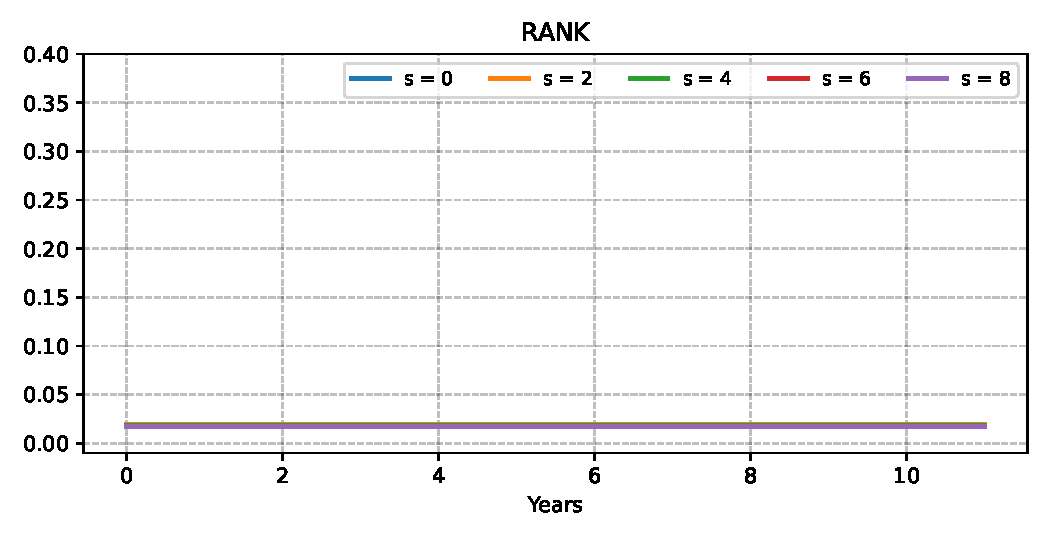
\includegraphics[width=0.5\linewidth]{figs/iMPC_RANK.pdf}
\end{figure}
\item <+->Flat and very low, about $0.02$ per year: far from the data
\end{itemize}
\end{frame}
%
\begin{frame}{Ricardian equivalence in RANK}
\begin{itemize}
\item <+->Recall that the deficit has zero present value for any $d\boldsymbol{G},d\boldsymbol{B}$: $\boldsymbol{q}^{\prime}(d\boldsymbol{G}-d\boldsymbol{T})=0$
\item <+->And it disappears in RANK:
\[
\boldsymbol{M}^{RA}(d\boldsymbol{G}-d\boldsymbol{T})=(1-\beta)\boldsymbol{1}\boldsymbol{q}^{\prime}(d\boldsymbol{G}-d\boldsymbol{T})=\boldsymbol{0}
\]
\item <+->Hence $d\boldsymbol{C}=\boldsymbol{0}$ and $d\boldsymbol{Y}=d\boldsymbol{G}$ for any $d\boldsymbol{G},d\boldsymbol{B}$
\item <+->\textbf{Impact and cumulative multipliers are exactly 1}, whatever the financing
\end{itemize}
\end{frame}
%
\begin{frame}{Ricardian equivalence: intuition}
\begin{itemize}
\item <+->The representative household smooths consumption perfectly
\item <+->It only cares about \textbf{permanent income}
\item <+->The government can shift income through time, with debt
\item <+->But it does not change permanent income: a tax cut today is a tax rise later
\item <+->So consumption does not change
\end{itemize}
\end{frame}
%
\begin{frame}{Is RANK realistic?}
\begin{itemize}
\item <+->\textbf{MPCs are too low:} $0.02$ per year against about $0.5$ in the data
\item <+->\textbf{Households are too forward-looking:} income far in the future counts at its full present value
\item <+->\textbf{No borrowing constraint:} every household can smooth
\end{itemize}
\end{frame}
%

\section{TANK}

\begin{frame}{Household problem in TANK}
\begin{itemize}
\item <+->\textbf{Share $\lambda$: hand-to-mouth.} No savings, consume all income, $MPC=1$:
\[
C_{t}^{H}=Z_{t}
\]
\item <+->\textbf{Share $1-\lambda$: Ricardian.} Same problem as in RANK, hold all the bonds
\item <+->Same labor and same tax rate for both types, so $Z_{t}=Y_{t}-T_{t}$ for both
\item <+->\textbf{Aggregate consumption:}
\[
C_{t}^{hh}=\lambda Z_{t}+(1-\lambda)C_{t}^{R}
\]
\end{itemize}
\end{frame}
%
\begin{frame}{Block representation}
\ikcdag{Two types}{$C^{hh}(\boldsymbol{Z})$}
\begin{itemize}
\item <+->Same picture as RANK: only the content of the red box changes
\end{itemize}
\end{frame}
%
\begin{frame}{iMPC in TANK}
\begin{itemize}
\item <+->The $\boldsymbol{M}$ matrix is a weighted sum:
\[
\boldsymbol{M}^{TA}=(1-\lambda)\boldsymbol{M}^{RA}+\lambda\boldsymbol{I}
\]
\item <+->$C_{t}$ overweights income at date $t$, but only at that same date\\
\begin{figure}[H]
\centering
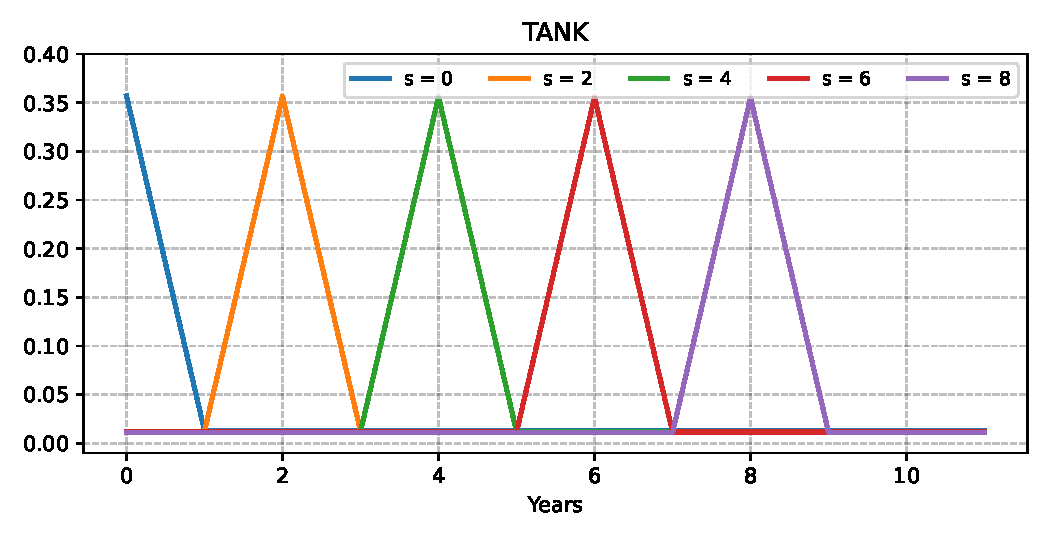
\includegraphics[width=0.7\linewidth]{figs/iMPC_TANK.pdf}
\end{figure}
\item <+->{\footnotesize{}Here $\lambda$ is set to match the annual MPC of baseline HANK}{\footnotesize\par}
\end{itemize}
\end{frame}
%
\begin{frame}{Solving TANK}
\begin{itemize}
\item <+->\textbf{Intertemporal Keynesian Cross} with $\boldsymbol{M}^{TA}$:
\begin{align*}
(\boldsymbol{I}-\boldsymbol{M}^{TA})d\boldsymbol{Y} & =d\boldsymbol{G}-\boldsymbol{M}^{TA}d\boldsymbol{T}\\
(\boldsymbol{I}-\boldsymbol{M}^{RA})d\boldsymbol{Y} & =\frac{1}{1-\lambda}\left[d\boldsymbol{G}-\lambda d\boldsymbol{T}\right]-\boldsymbol{M}^{RA}d\boldsymbol{T}
\end{align*}
\item <+->This is the RANK IKC with a modified spending shock. \textbf{Solution:}
\[
d\boldsymbol{Y}=d\boldsymbol{G}+\frac{\lambda}{1-\lambda}\left[d\boldsymbol{G}-d\boldsymbol{T}\right]
\]
\item <+->Same form as the IS-LM Keynesian cross, with $\lambda$ in the role of $c_{1}$
\item <+->Amplification with deficit financing, increasing in $\lambda$
\end{itemize}
\end{frame}
%
\begin{frame}{TANK Proof}
\begin{itemize}
\item {\footnotesize{}In TANK we have:
\begin{align*}
d\boldsymbol{Y} & =d\boldsymbol{G}+\boldsymbol{M}^{TA}\left(d\boldsymbol{Y}-d\boldsymbol{T}\right)\\
(\boldsymbol{I}-\boldsymbol{M}^{TA})d\boldsymbol{Y} & =d\boldsymbol{G}-\boldsymbol{M}^{TA}d\boldsymbol{T}\\
(\boldsymbol{I}-\boldsymbol{M}^{RA})d\boldsymbol{Y} & =\frac{1}{1-\lambda}\left[d\boldsymbol{G}-\lambda d\boldsymbol{T}\right]-\boldsymbol{M}^{RA}d\boldsymbol{T}\\
d\boldsymbol{Y} & =\boldsymbol{M}^{RA}d\boldsymbol{Y}-\boldsymbol{M}^{RA}d\boldsymbol{T}+\frac{1}{1-\lambda}\left[d\boldsymbol{G}-\lambda d\boldsymbol{T}\right]\\
d\boldsymbol{Y} & =d\tilde{\boldsymbol{G}}+\boldsymbol{M}^{RA}\left(d\boldsymbol{Y}-d\boldsymbol{T}\right)
\end{align*}
}{\footnotesize\par}
\item {\footnotesize{}where $d\tilde{\boldsymbol{G}}=\frac{1}{1-\lambda}\left[d\boldsymbol{G}-\lambda d\boldsymbol{T}\right]$}{\footnotesize\par}
\item {\footnotesize{}Recall that in RANK $d\boldsymbol{Y}=d\boldsymbol{G}+\boldsymbol{M}^{RA}(d\boldsymbol{Y}-d\boldsymbol{T})$
with solution $d\boldsymbol{Y}=d\boldsymbol{G}$ thus implying $d\boldsymbol{Y}=d\tilde{\boldsymbol{G}}$
in TANK:
\begin{align*}
d\boldsymbol{Y} & =\frac{1}{1-\lambda}\left[d\boldsymbol{G}-\lambda d\boldsymbol{T}\right]\\
d\boldsymbol{Y} & =d\boldsymbol{G}-d\boldsymbol{G}+\frac{1}{1-\lambda}\left[d\boldsymbol{G}-\lambda d\boldsymbol{T}\right]\\
d\boldsymbol{Y} & =d\boldsymbol{G}+\frac{\lambda}{1-\lambda}\left[d\boldsymbol{G}-d\boldsymbol{T}\right]
\end{align*}
}{\footnotesize\par}
\end{itemize}
\end{frame}
%
\begin{frame}{Impact and cumulative multipliers in TANK}
\begin{itemize}
\item <+->\textbf{Impact multiplier} if debt absorbs all of the spending at $t=0$, so $dT_{0}=0$:
\[
\frac{dY_{0}}{dG_{0}}=\frac{1}{1-\lambda}>1
\]
\item <+->\textbf{Cumulative multiplier} is still one:
\begin{align*}
\frac{\boldsymbol{q}^{\prime}d\boldsymbol{Y}}{\boldsymbol{q}^{\prime}d\boldsymbol{G}} & =\frac{\boldsymbol{q}^{\prime}d\boldsymbol{G}+\frac{\lambda}{1-\lambda}\boldsymbol{q}^{\prime}\left[d\boldsymbol{G}-d\boldsymbol{T}\right]}{\boldsymbol{q}^{\prime}d\boldsymbol{G}}=1
\end{align*}
\item <+->The boom on impact is exactly offset by the bust when taxes are repaid
\end{itemize}
\end{frame}
%
\begin{frame}{What TANK misses}
\begin{itemize}
\item <+->$dC_{t}$ depends only on the deficit at the same date
\begin{itemize}
\item No persistence: the boost ends when the deficit ends
\item Consumption falls during repayment
\end{itemize}
\item <+->No intertemporal MPCs: it can match the MPC on impact, but $M_{1,0}$ is far too low
\item <+->Stylized level of inequality
\item <+->Hard to connect to micro data
\item <+->No precautionary saving
\end{itemize}
\end{frame}
%
\begin{frame}{Exercise: RANK and TANK}
The code is in \emph{Exercise-RANK}. Shock: $dG$ with $dB_{t}=\rho_{B}(dB_{t-1}+dG_{t})$.
\begin{enumerate}
\item {\small Read the model equations in \emph{blocks.py}. Check that they match the IKC model in RANK and TANK.}
\item {\small Solve for the IRF to a government spending shock in RANK with \emph{model.find\_IRFs()}. Compare with the analytical formula.}
\item {\small Compute the impact and cumulative multipliers in RANK. What feature of the household block explains this result?}
\item {\small Solve for the IRF to a government spending shock in TANK ($\lambda=0.3$) with \emph{model.find\_IRFs()}. Compare with the analytical formula.}
\item {\small Compute the impact and cumulative multipliers in TANK. What feature of the household block explains this result?}
\item {\small Compute the impact and cumulative multipliers for $\lambda\in\{0,0.1,\dots,0.5\}$, and discuss.}
\item {\small Compute the inflation response in RANK and TANK. Does inflation affect the output response? Why?}
\end{enumerate}
\end{frame}
%

\section{HANK}

\begin{frame}{Household problem in HANK}
\begin{itemize}
\item \textbf{Household problem:}
\begin{align*}
v_{t}(z_{t},a_{t-1}) & =\max_{c_{t}}\frac{c_{t}^{1-\sigma}}{1-\sigma}-\varphi\frac{\ell_{t}^{1+\nu}}{1+\nu}+\beta\mathbb{E}_{t}\left[v_{t+1}(z_{t+1},a_{t})\right]\\
\text{s.t. }a_{t}+c_{t} & =(1+r_{t}^{p})a_{t-1}+\left(1-\tau_{t}\right)w_{t}\ell_{t}z_{t}+\chi_{t}\\
\log z_{t+1} & =\rho_{z}\log z_{t}+\psi_{t+1}\,\,\,,\psi_{t}\sim\mathcal{N}(\mu_{\psi},\sigma_{\psi}),\,\mathbb{E}[z_{t}]=1\\
a_{t} & \geq0
\end{align*}
\item \textbf{Active decisions:} Consumption-saving, $c_{t}$ (and $a_{t}$)
\item \textbf{Union decision:} Labor supply, $\ell_{t}$
\item \textbf{Aggregate Consumption: $C_{t}^{hh}=\int c_{t}d\mathcal{D}_{t}$}
\item \textbf{Consumption function: $\boldsymbol{C}^{hh}=C^{hh}(\boldsymbol{Z},\boldsymbol{r}^{p})$} with $Z_{t}=\left(1-\tau_{t}\right)w_{t}\ell_{t}$ and transfers $\chi_{t}=0$ at baseline
\end{itemize}
\end{frame}
%
\begin{frame}{Block representation}
\ikcdag{Heterogeneous}{$C^{hh}(\boldsymbol{Z})$}
\begin{itemize}
\item <+->$C^{hh}(\boldsymbol{Z})$ is unchanged as an object
\item <+->We now compute it from the distribution of households
\end{itemize}
\end{frame}
%
\begin{frame}{iMPC in HANK}
\begin{itemize}
\item <+->$\boldsymbol{M}$ is computed numerically: the household Jacobian with respect to $Z$, as in lectures 5-6\\
\begin{figure}[H]
\centering
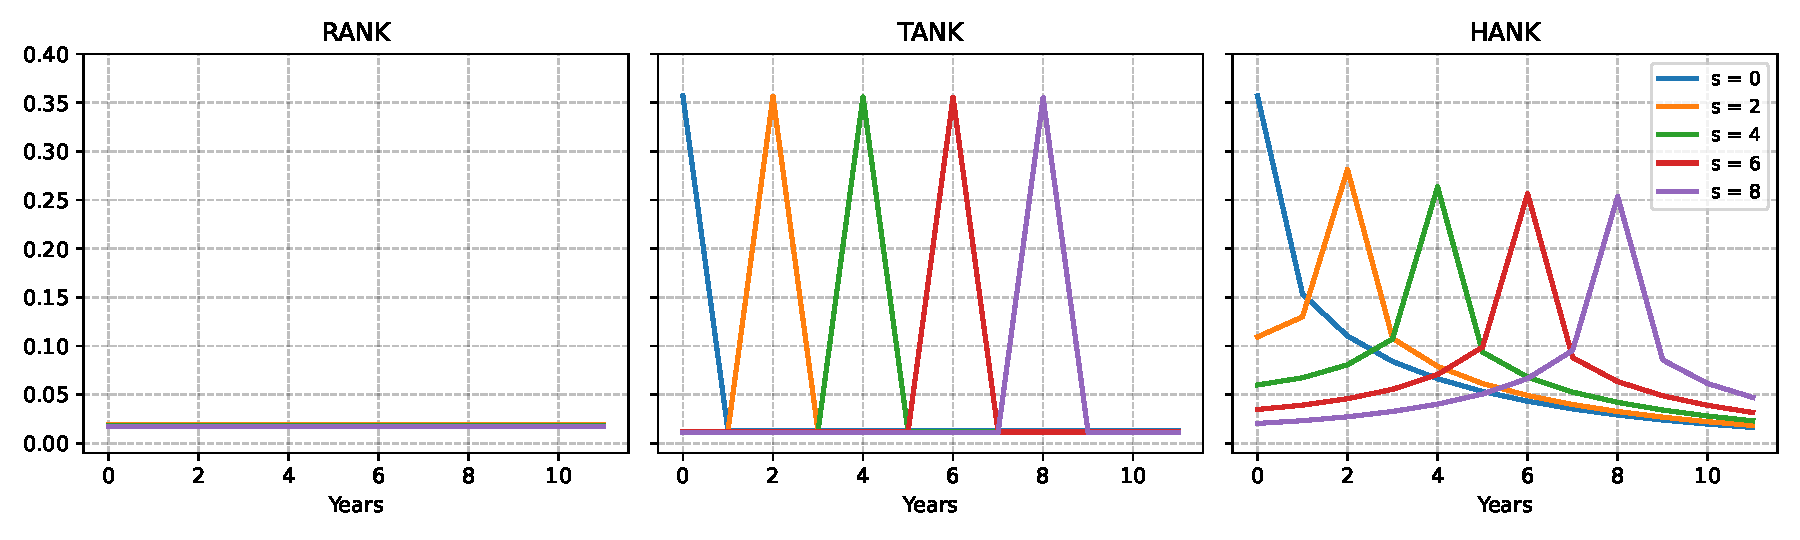
\includegraphics[width=0.95\linewidth]{figs/iMPC_compare.pdf}
\end{figure}
\item <+->Spending is spread around the date of the income: anticipated before, gradual after
\item <+->Past and future income matter at all horizons, not only the same date
\end{itemize}
\end{frame}
%
\begin{frame}{iMPCs in the data: yes!}
\begin{figure}[H]
\centering
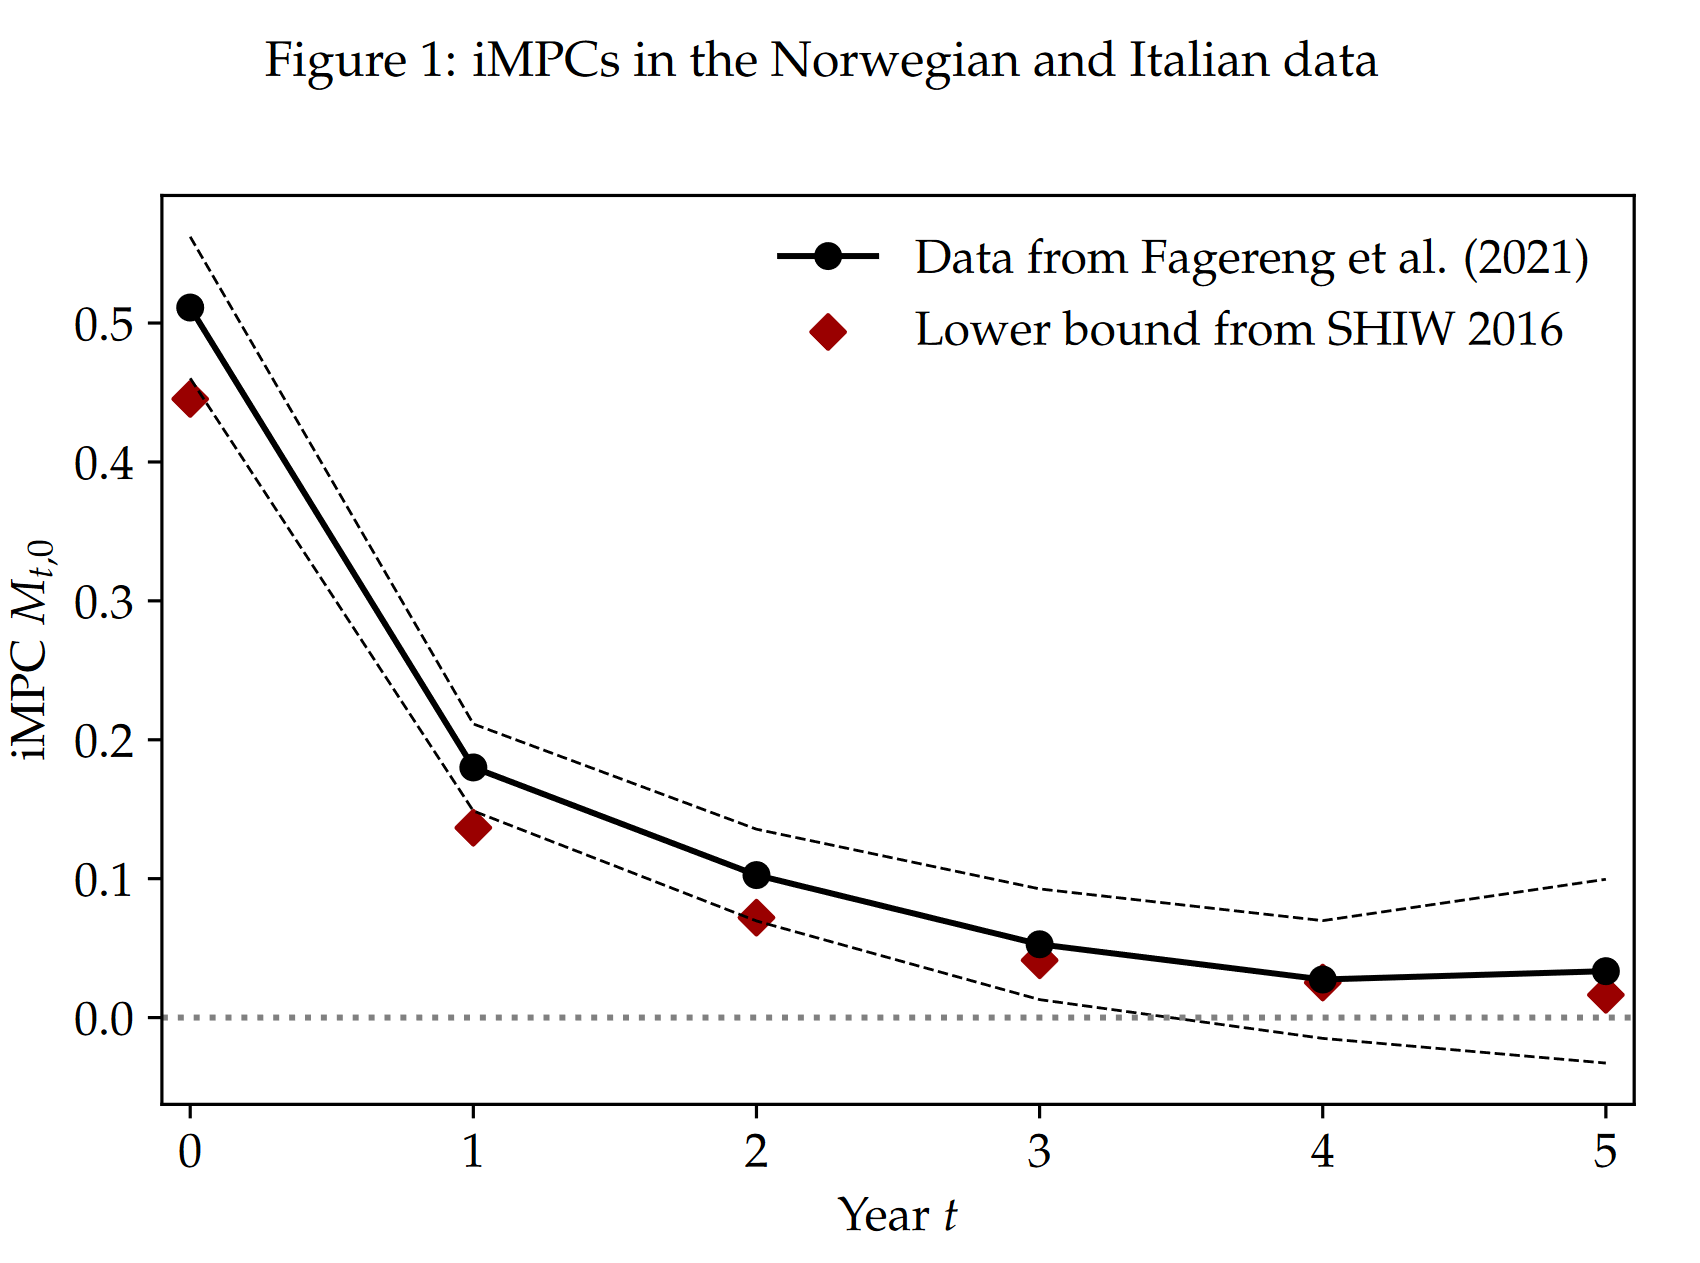
\includegraphics[width=0.45\linewidth]{figs/iMPC_data.png}
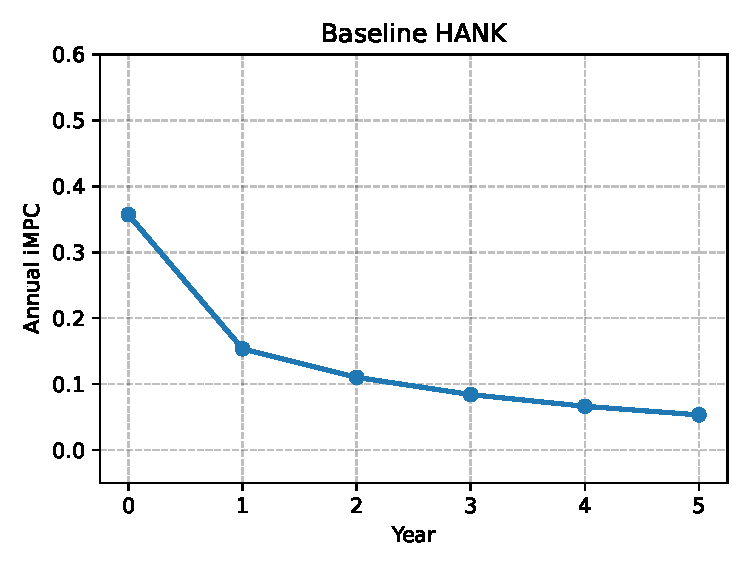
\includegraphics[width=0.45\linewidth]{figs/iMPC_annual.pdf}
\end{figure}
\begin{itemize}
\item <+->Same shape: high on impact, then a gradual decline
\item <+->Baseline model: 0.36 and 0.15. Data: 0.51 and 0.18
\item <+->RANK has no decline, TANK has a drop after one period
\item <+->We only observe the first column, the rest comes from the model
\end{itemize}
\end{frame}
%
\begin{frame}{Consumption function in HANK}
\begin{figure}[H]
\centering
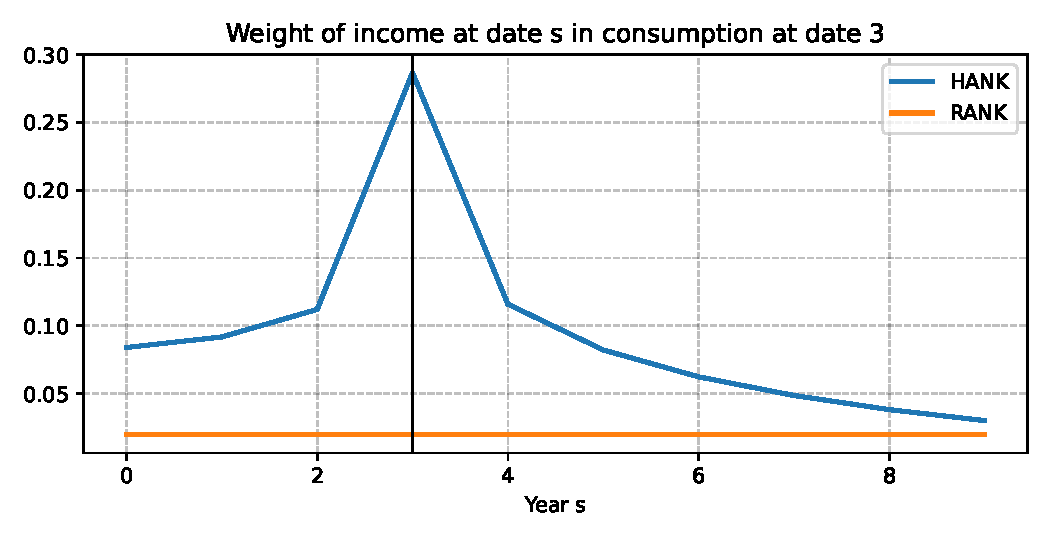
\includegraphics[width=0.48\linewidth]{figs/M_row.pdf}
\end{figure}
\begin{itemize}
\item <+->Present value weights $M_{3,s}(1+r)^{s}$ peak at date 3. They are flat in RANK
\item <+->Two properties:
\begin{enumerate}
\item \textbf{Front-loaded:} income is spent soon after it arrives
\item \textbf{Discounted:} households react less to future changes than the present value implies
\end{enumerate}
\end{itemize}
\end{frame}
%
\begin{frame}{Why this breaks Ricardian equivalence}
\begin{itemize}
\item <+->With $D_{s}=dG_{s}-dT_{s}$, the first round of spending is
\[
\sum_{s}M_{t,s}D_{s}=\sum_{s}\underset{\text{weight}}{\underbrace{M_{t,s}(1+r_{ss})^{s}}}q_{s}D_{s}
\]
\item <+->\textbf{Flat weights (RANK):} the sum is proportional to $\boldsymbol{q}^{\prime}\boldsymbol{D}=0$, so deficits are neutral
\item <+->\textbf{Peaked weights (HANK):} larger weights on the early deficit than on the later repayment give a boost
\item <+->So the timing of income matters, not just its present value
\end{itemize}
\end{frame}
%
\begin{frame}{HANK: deficit-financed spending shock}
\begin{figure}[H]
\centering
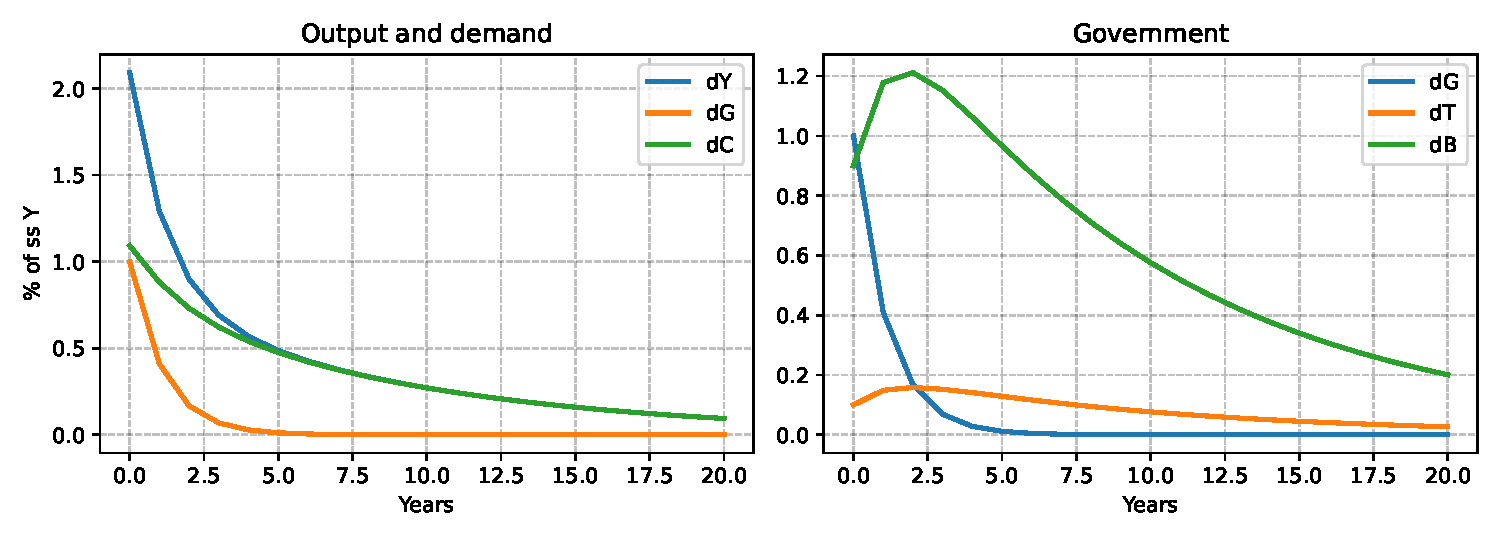
\includegraphics[width=0.85\linewidth]{figs/fiscal_irf.pdf}
\end{figure}
\vspace{-2mm}
\begin{itemize}
\item <+->Output rises by twice the spending on impact: consumption rises as much as $G$
\item <+->Taxes rise slowly, so debt keeps rising for two years, then decays
\item <+->Consumption stays high as long as debt is high: a persistent boom
\end{itemize}
\end{frame}
%
\begin{frame}{Rounds of spending}
\begin{itemize}
\item <+->My income is your spending, spread over time:
\[
d\boldsymbol{C}=\sum_{k\geq1}\boldsymbol{M}^{k}(d\boldsymbol{G}-d\boldsymbol{T})
\]
\end{itemize}
\begin{figure}[H]
\centering
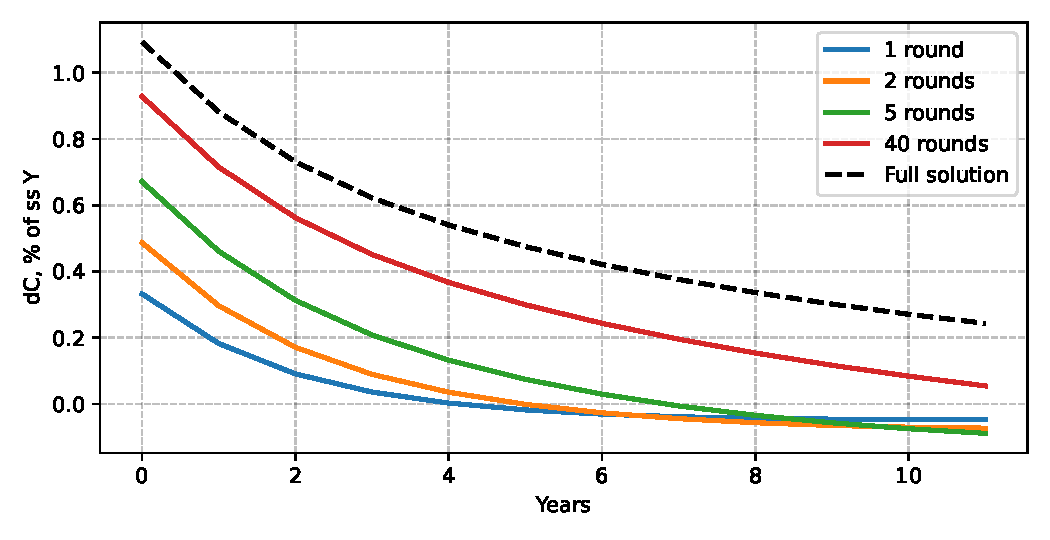
\includegraphics[width=0.58\linewidth]{figs/rounds.pdf}
\end{figure}
\begin{itemize}
\item <+->The first round explains most of the impact
\item <+->Later rounds explain the persistence
\end{itemize}
\end{frame}
%
\begin{frame}{Multipliers and debt persistence}
\begin{figure}[H]
\centering
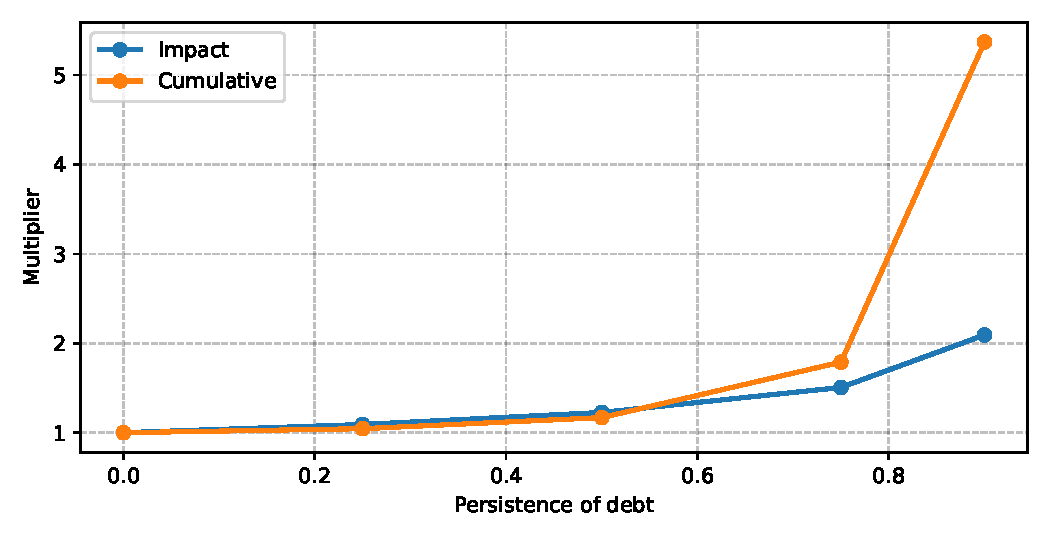
\includegraphics[width=0.5\linewidth]{figs/multipliers_rho_B.pdf}
\end{figure}
\vspace{-2mm}
\begin{itemize}
\item <+->Debt path: $dB_{t}=\rho_{B}\left(dB_{t-1}+dG_{t}\right)$, and taxes follow from the budget
\item <+->More persistent debt means larger multipliers, on impact and cumulatively
\item <+->Aggregate estimates are 0.6-0.8, and the data does not reject up to 1.5 (Ramey, 2019)
\end{itemize}
\end{frame}
%
\begin{frame}{Why is the cumulative multiplier above 1?}
\begin{itemize}
\item <+->\textbf{TANK:} Ricardian households hold any amount of debt at $r_{ss}$. Debt needs no boom, so $\boldsymbol{q}^{\prime}d\boldsymbol{C}=0$
\item <+->\textbf{HANK:} households must want to hold the extra debt. At fixed $r$, only higher income makes them want more assets
\item <+->So \textbf{persistent debt needs a persistent boom}
\begin{itemize}
\item Baseline with $\rho_{B}=0.9$: long after $dG_{t}$ is gone, $dY_{t}\approx0.47\,dB_{t}$
\item More persistent debt lasts longer, so the boom lasts longer
\end{itemize}
\end{itemize}
\end{frame}
%
\begin{frame}{Takeaway}
\begin{itemize}
\item <+->Multipliers on deficit-financed $G$, at constant $r$:
\end{itemize}
\vspace{2mm}
\begin{center}
\begin{tabular}{lccc}
 & \textbf{Ricardian equivalence} & \textbf{Impact} & \textbf{Cumulative}\\
\hline
\textbf{RANK} & yes & $1$ & $1$\\
\textbf{TANK} & no & $>1$ & $1$\\
\textbf{HANK} & no & $>1$ & $>1$\\
\end{tabular}
\end{center}
\vspace{2mm}
\begin{itemize}
\item <+->Same macro blocks: only the household block, and so $\boldsymbol{M}$, changes
\end{itemize}
\end{frame}
%

\section{Self-financing deficits}

\begin{frame}{Self-financing deficits}
\begin{itemize}
\item <+->So far the debt path is chosen and the tax rate adjusts. Now the reverse (Angeletos, Lian and Wolf, 2024): \textbf{$\tau$ stays fixed and debt adjusts}
\item <+->A rise in $G$ is financed by debt, and no tax hike ever comes: $d\boldsymbol{T}=\tau d\boldsymbol{Y}$
\item <+->The IKC becomes
\[
d\boldsymbol{Y}=d\boldsymbol{G}+(1-\tau)\boldsymbol{M}d\boldsymbol{Y}\quad\Leftrightarrow\quad\left(\boldsymbol{I}-(1-\tau)\boldsymbol{M}\right)d\boldsymbol{Y}=d\boldsymbol{G}
\]
\item <+->With $\tau>0$ the inverse can exist, unlike $\boldsymbol{I}-\boldsymbol{M}$: rounds die out because the government takes $\tau$ of each one
\item <+->Multiply by $\boldsymbol{q}^{\prime}$ and use $\boldsymbol{q}^{\prime}\boldsymbol{M}=\boldsymbol{q}^{\prime}$:
\[
\tau\boldsymbol{q}^{\prime}d\boldsymbol{Y}=\boldsymbol{q}^{\prime}d\boldsymbol{G}\quad\Leftrightarrow\quad\frac{\boldsymbol{q}^{\prime}d\boldsymbol{Y}}{\boldsymbol{q}^{\prime}d\boldsymbol{G}}=\frac{1}{\tau}
\]
\item <+->The cumulative multiplier is exactly $1/\tau$: new tax revenue repays the whole spending
\end{itemize}
\end{frame}
%
\begin{frame}{Self-financing deficits: illustration}
\begin{figure}[H]
\centering
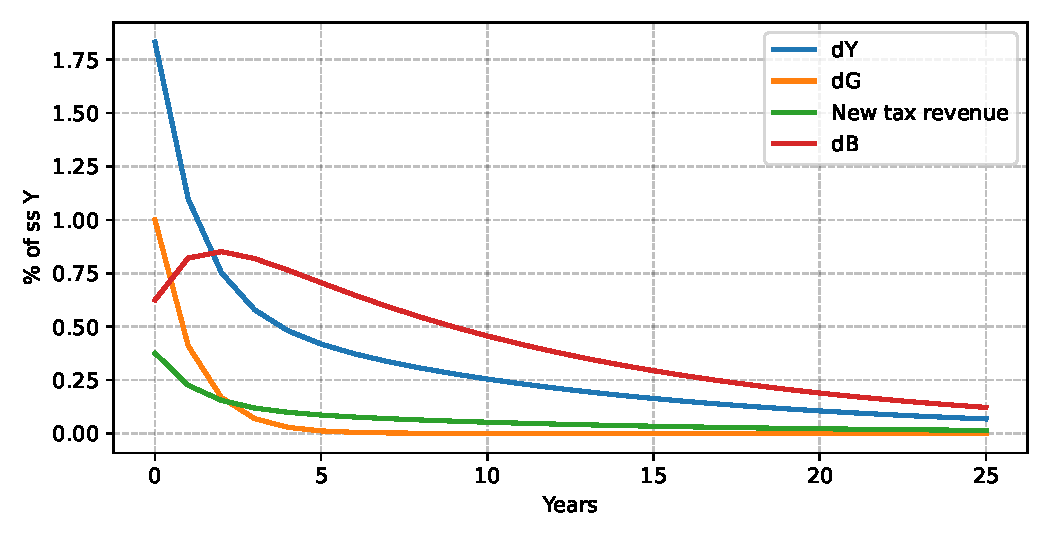
\includegraphics[width=0.62\linewidth]{figs/self_financing.pdf}
\end{figure}
\begin{itemize}
\item <+->Debt rises, then returns to steady state without any tax hike
\item <+->This needs rows of $\boldsymbol{M}$ that decline. In RANK, output rises forever and debt never returns
\item <+->{\footnotesize{}Holds at constant $r$. With nominal debt, inflation also erodes part of the debt}{\footnotesize\par}
\end{itemize}
\end{frame}
%
\begin{frame}{How much of a deficit is self-financed?}
\begin{itemize}
\item <+->For any debt path, taxes must repay the spending: $\boldsymbol{q}^{\prime}d\boldsymbol{T}=\boldsymbol{q}^{\prime}d\boldsymbol{G}$
\item <+->Taxes rise with the tax base and with the tax rate: $dT_{t}\approx\tau_{ss}dY_{t}+Y_{ss}d\tau_{t}$, so
\[
Y_{ss}\boldsymbol{q}^{\prime}d\boldsymbol{\tau}=\left(1-\tau_{ss}\times\frac{\boldsymbol{q}^{\prime}d\boldsymbol{Y}}{\boldsymbol{q}^{\prime}d\boldsymbol{G}}\right)\boldsymbol{q}^{\prime}d\boldsymbol{G}
\]
\item <+->\textbf{Self-financed share:} $\tau_{ss}\times$ cumulative multiplier
\item <+->\textbf{Cumulative multiplier above $1/\tau_{ss}$:} the deficit is fully self-financed, and the tax rate can even fall
\item <+->\textbf{Baseline:} $1/\tau_{ss}\approx4.9$
\begin{itemize}
\item $\rho_{B}=0.75$: multiplier 1.8, so 37\% is self-financed
\item $\rho_{B}=0.9$: multiplier 5.4, so 110\%
\end{itemize}
\item <+->Persistent debt is what makes self-financing possible
\item <+->\textbf{How robust is this?} All of this is at a constant $r$. With a Taylor rule, the cumulative multiplier falls (to 0.43 in the canonical model, see later), and so does self-financing
\end{itemize}
\end{frame}
%

\section{Liquidity}

\begin{frame}{Liquidity: low liquidity}
\begin{itemize}
\item <+->So far the only asset is government bonds
\item <+->Low liquid wealth gives high MPCs: calibrating $B/Y$ to an annual MPC of about 0.5 gives roughly the amount of liquid wealth in the data
\item <+->The baseline model is of this type: $B=0.25$ of annual output, with an annual MPC of 0.36
\item <+->Called HA-one in Auclert et al.
\end{itemize}
\end{frame}
%
\begin{frame}{Liquidity: high wealth}
\begin{itemize}
\item <+->But total wealth in the data is much larger
\item <+->Assume $\mu>1$ and match $(p+B)/Y=500\%$ of annual GDP
\item <+->Then MPCs are \textbf{too low}: households have enough assets to smooth income shocks
\item <+->\textbf{Solution:} heterogeneous $\beta$, in Auclert, Rognlie and Straub (2025)
\begin{itemize}
\item Rich households hold most of the wealth
\item The bottom 90\% have higher MPCs and little wealth
\end{itemize}
\end{itemize}
\end{frame}
%
\begin{frame}{Liquidity: two assets}
\begin{itemize}
\item <+->\textbf{Other solution:} two-asset models with high total wealth (Auclert et al.; Kaplan, Moll and Violante)
\item <+->\textbf{Wealthy hand-to-mouth} households: positive net worth but low liquid wealth (housing)
\item <+->Match high wealth and high MPCs
\item <+->Called HA-two in Auclert et al.
\end{itemize}
\end{frame}
%
\begin{frame}{Back to the data}
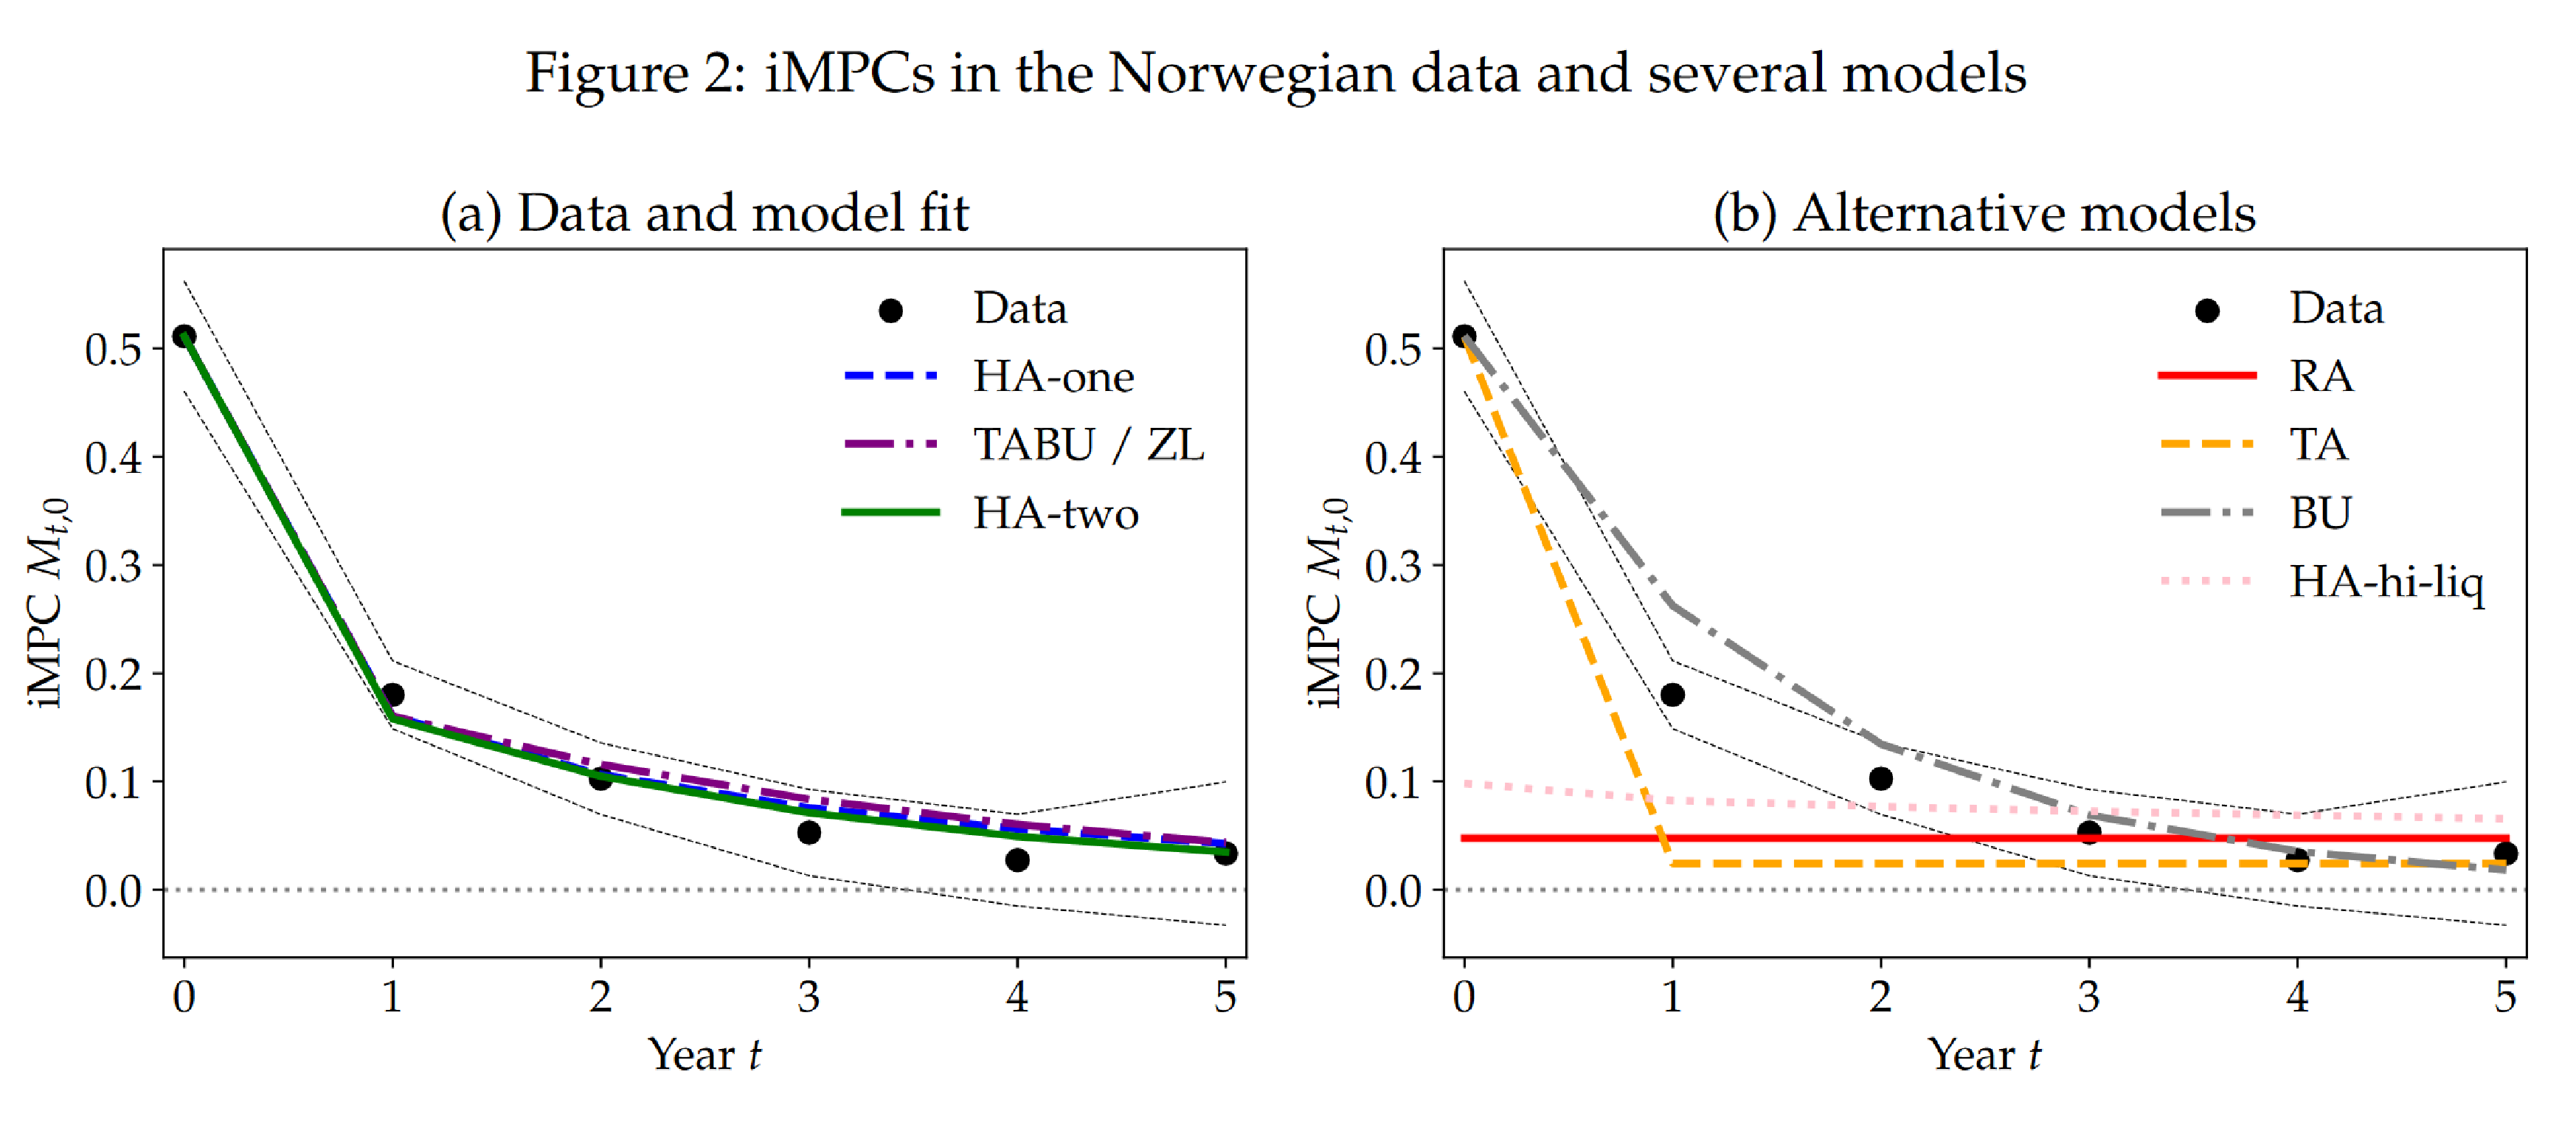
\includegraphics[width=1\textwidth]{figs/iMPC_models}
\begin{itemize}
\item <+->HA-one and HA-two fit the first column
\item <+->HA-hi-liq, a one-asset model at high wealth, does not. Neither does RA or TA
\end{itemize}
\end{frame}
%
\begin{frame}{Back to multipliers}
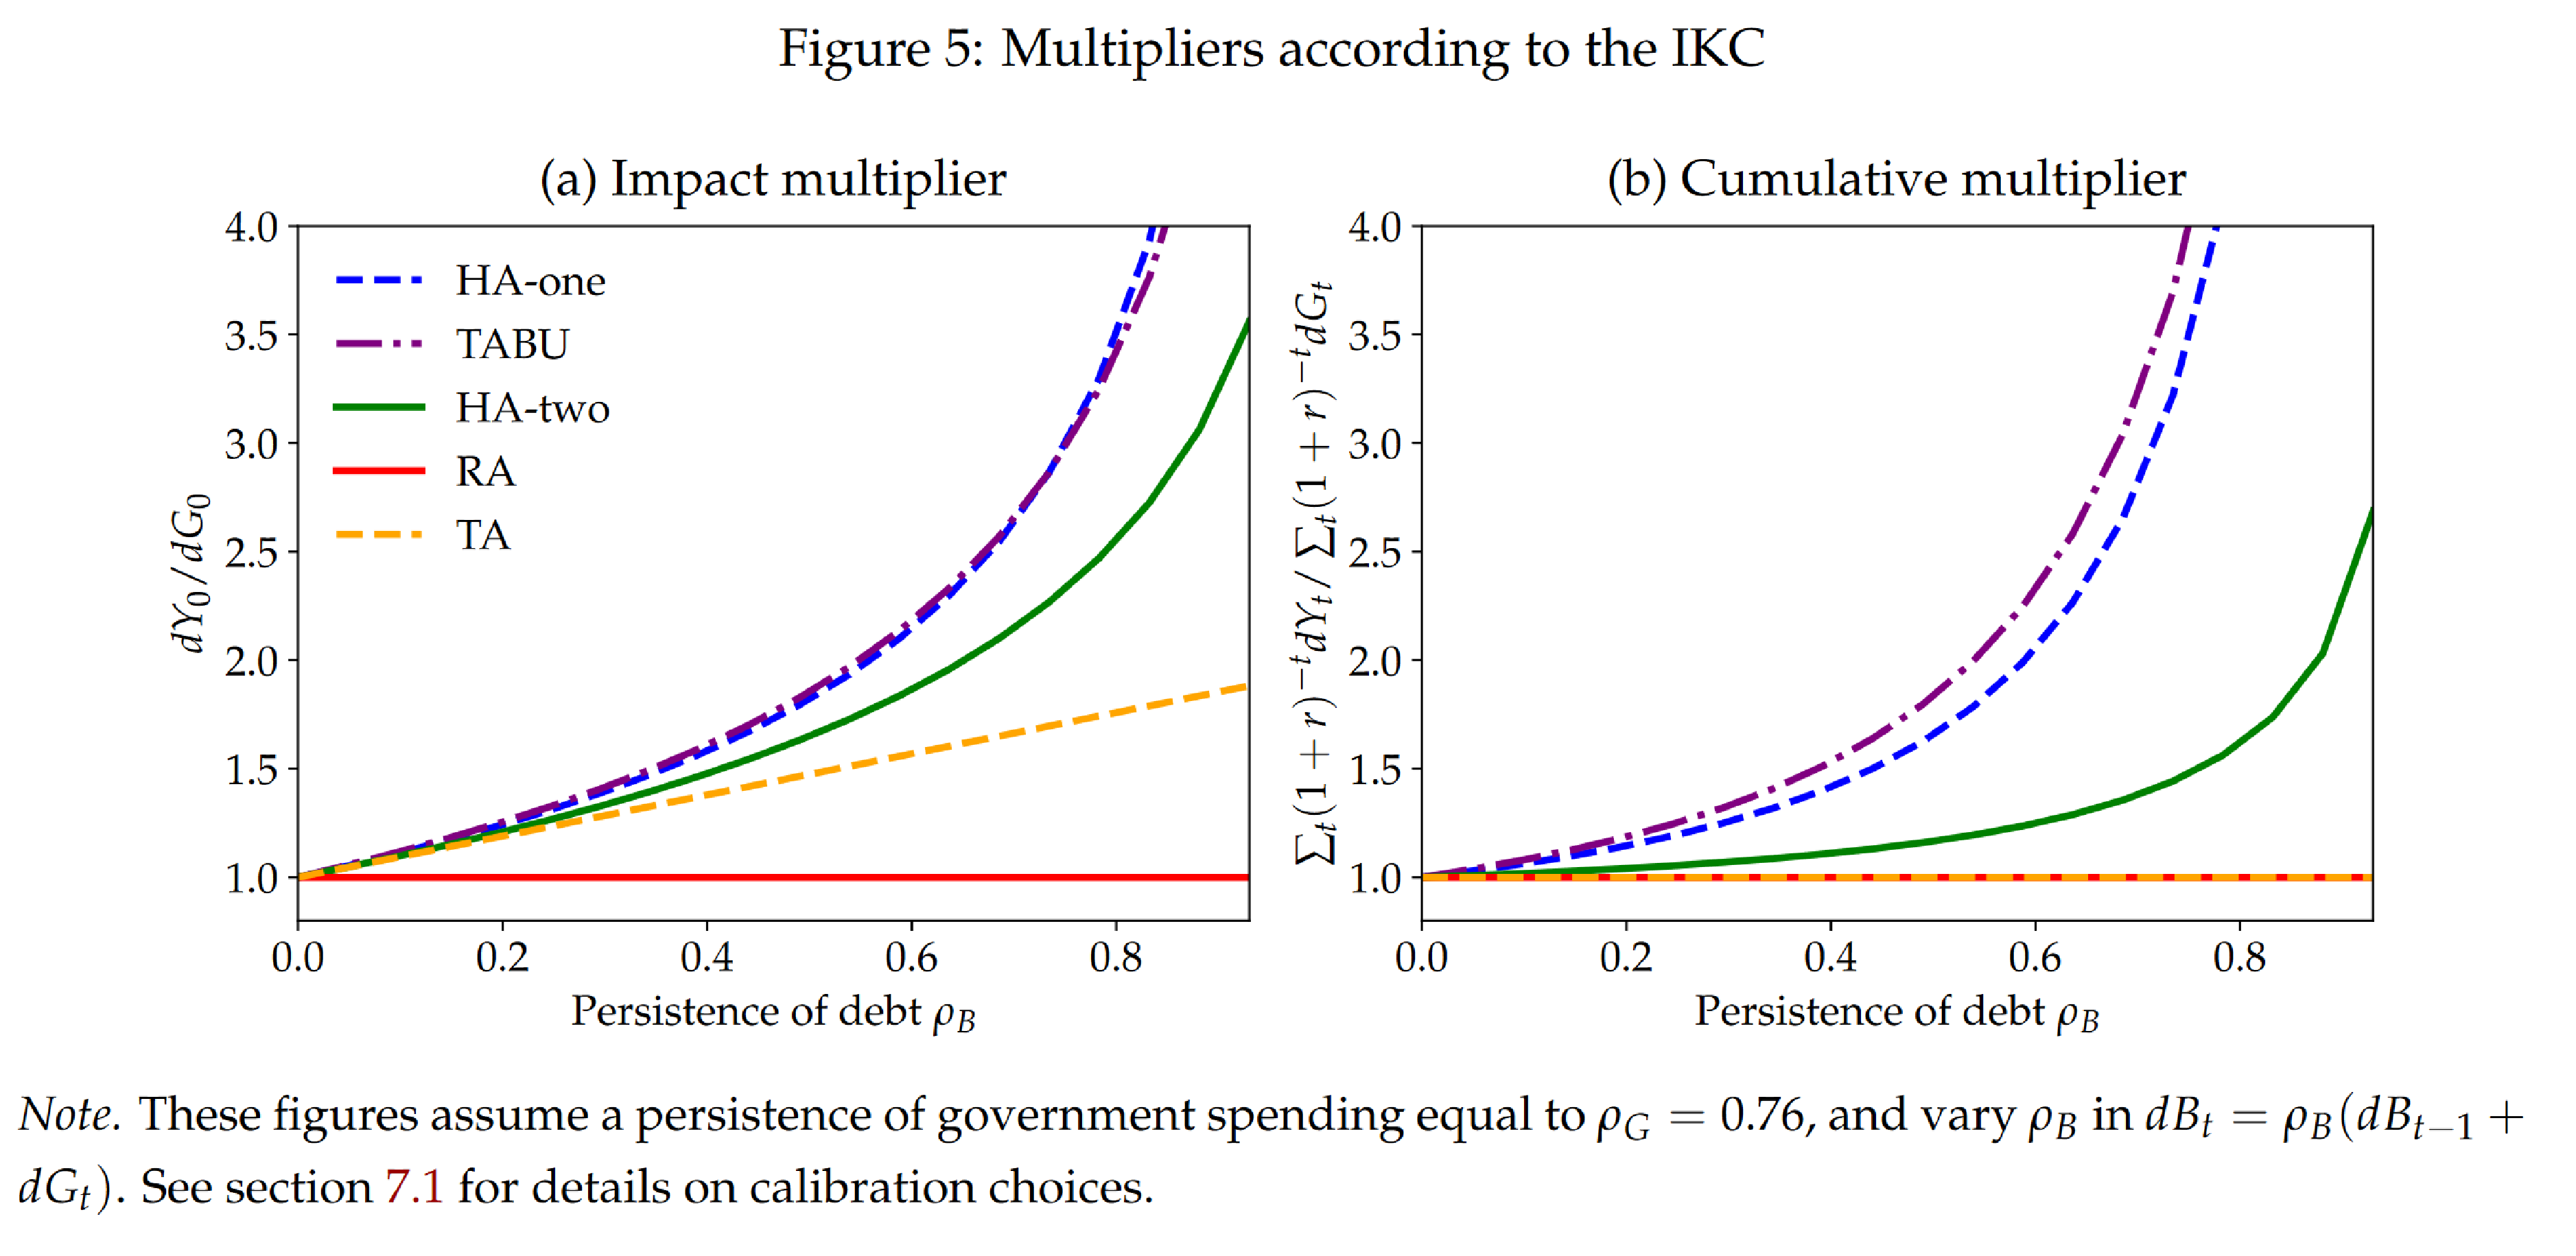
\includegraphics[width=1\textwidth]{figs/multiplier}
\begin{itemize}
\item <+->Models that fit the iMPCs have similar impact multipliers
\item <+->Cumulative multipliers are above 1 in both, but much lower in HA-two: savings migrate to the illiquid account, so iMPCs decline more slowly
\end{itemize}
\end{frame}
%

\section{Generalized IKC}

\begin{frame}{Generalized IKC}
\begin{itemize}
\item <+->So far: real rate rule, real bonds, $\mu=1$
\item <+->We now drop these assumptions one at a time, starting each time from the IKC:
\begin{enumerate}
\item \textbf{Markups:} $\mu>1$, so $p>0$ and capital gains
\item \textbf{Taylor rule:} inflation moves $r$, so we need the W-NKPC
\item \textbf{Nominal bonds:} surprise inflation revalues debt at $t=0$
\end{enumerate}
\item <+->Then we put all of them together
\end{itemize}
\end{frame}
%
\begin{frame}{1. Markups: consumption depends on capital gains}
\begin{itemize}
\item <+->With $\mu>1$, income is split in two:
\[
Z_{t}=\frac{1}{\mu}\left(Y_{t}-T_{t}\right),\quad d_{t}=\left(1-\frac{1}{\mu}\right)\left(Y_{t}-T_{t}\right)
\]
\item <+->Households receive $Z_{t}$ directly. Dividends go through the mutual fund: a shock at $t=0$ changes all expected dividends, so the stock price jumps
\item <+->\textbf{Capital gain:} the first-period return pays this out in one go, with real bonds
\[
\text{cap}_{0}\equiv A_{ss}dr_{0}^{p}=dp_{0}+dd_{0}
\]
\item <+->\textbf{Consumption} reacts to both, with $\boldsymbol{m}=\partial\boldsymbol{C}^{hh}/\partial\text{cap}_{0}$ the iMPCs out of capital gains:
\[
d\boldsymbol{C}=\frac{1}{\mu}\boldsymbol{M}\left(d\boldsymbol{Y}-d\boldsymbol{T}\right)+\boldsymbol{m}\text{cap}_{0}
\]
\item <+->\textbf{Goal:} write $\text{cap}_{0}$ as a function of $d\boldsymbol{Y}$ and $d\boldsymbol{T}$
\end{itemize}
\end{frame}
%
\begin{frame}{1. Markups: capital gain as a function of $d\boldsymbol{Y}$}
\vspace{-1mm}
\begin{itemize}
\item <+->\textbf{Step 1:} no arbitrage at constant $r$: $p_{t}=\frac{p_{t+1}+d_{t+1}}{1+r_{ss}}$
\item <+->\textbf{Step 2:} iterate forward from $t=0$, with $q_{t}=(1+r_{ss})^{-t}$ and no bubble. The stock price is the present value of dividends:
\[
p_{0}+d_{0}=\sum_{t=0}^{\infty}q_{t}d_{t}=\boldsymbol{q}^{\prime}\boldsymbol{d}
\]
\item <+->\textbf{Step 3:} differentiate at constant $r$, so $\boldsymbol{q}$ does not move:
\[
\text{cap}_{0}=dp_{0}+dd_{0}=\boldsymbol{q}^{\prime}d\boldsymbol{d}
\]
\item <+->\textbf{Step 4:} use $d\boldsymbol{d}=\left(1-\frac{1}{\mu}\right)\left(d\boldsymbol{Y}-d\boldsymbol{T}\right)$:
\[
\text{cap}_{0}=\left(1-\frac{1}{\mu}\right)\boldsymbol{q}^{\prime}\left(d\boldsymbol{Y}-d\boldsymbol{T}\right)
\]
\end{itemize}
\end{frame}
%
\begin{frame}{1. Markups: IKC with capital gains}
\begin{itemize}
\item <+->Replace $\text{cap}_{0}$ in consumption, and use $d\boldsymbol{Y}=d\boldsymbol{C}+d\boldsymbol{G}$:
\[
d\boldsymbol{Y}=d\boldsymbol{G}+\bar{\boldsymbol{M}}\left(d\boldsymbol{Y}-d\boldsymbol{T}\right),\quad\bar{\boldsymbol{M}}\equiv\frac{1}{\mu}\boldsymbol{M}+\left(1-\frac{1}{\mu}\right)\boldsymbol{m}\boldsymbol{q}^{\prime}
\]
\item <+->\textbf{Same IKC:} $\bar{\boldsymbol{M}}$ is an average of two iMPCs, out of labor income and out of capital gains
\item <+->Still $\boldsymbol{q}^{\prime}\bar{\boldsymbol{M}}=\boldsymbol{q}^{\prime}$, since $\boldsymbol{q}^{\prime}\boldsymbol{m}=1$: a capital gain is eventually fully spent
\item <+->So everything holds with $\bar{\boldsymbol{M}}$: the balanced budget multiplier is 1, and RANK is unchanged since $\boldsymbol{m}\boldsymbol{q}^{\prime}=\boldsymbol{M}^{RA}$
\item <+->$\boldsymbol{m}$ is small: profits go to wealthy households with low MPCs, so $\bar{\boldsymbol{M}}$ is below $\boldsymbol{M}$ on impact
\end{itemize}
\end{frame}
%
\begin{frame}{2. Taylor rule: $r$ moves}
\begin{itemize}
\item <+->Back to $\mu=1$ and real bonds, now with $i_{t}=i_{ss}+\phi\pi_{t}$
\item <+->\textbf{Real rate:} from the Taylor rule and Fisher, with $\boldsymbol{F}$ the lead matrix:
\[
d\boldsymbol{r}=\left(\phi\boldsymbol{I}-(1+r_{ss})\boldsymbol{F}\right)d\boldsymbol{\pi}
\]
\item <+->\textbf{Consumption} reacts to $r$, with $\boldsymbol{M}^{r}=\partial\boldsymbol{C}^{hh}/\partial\boldsymbol{r}$:
\[
d\boldsymbol{Y}=d\boldsymbol{G}+\boldsymbol{M}\left(d\boldsymbol{Y}-d\boldsymbol{T}\right)+\boldsymbol{M}^{r}d\boldsymbol{r}
\]
\item <+->\textbf{Taxes} also pay the interest on debt, which is now moving:
\[
d\boldsymbol{T}=d\boldsymbol{G}-\left(\boldsymbol{I}-(1+r_{ss})\boldsymbol{L}\right)d\boldsymbol{B}+B_{ss}\boldsymbol{L}d\boldsymbol{r}
\]
\item <+->Output now depends on inflation, so the W-NKPC is no longer a side equation
\end{itemize}
\end{frame}
%
\begin{frame}{2. Taylor rule: two vector equations}
\begin{itemize}
\item <+->\textbf{Linearize the W-NKPC} around steady state, with $Y_{ss}=1$:
\[
d\boldsymbol{\pi}=\boldsymbol{K}\left(\nu d\boldsymbol{Y}+\frac{\sigma}{C_{ss}}\left(d\boldsymbol{Y}-d\boldsymbol{G}\right)+\frac{d\boldsymbol{\tau}}{1-\tau_{ss}}\right),\quad\boldsymbol{K}\equiv\kappa h'(1)\left(\boldsymbol{I}-\beta\boldsymbol{F}\right)^{-1}
\]
with $\nu$ the inverse Frisch elasticity, $\sigma$ the inverse EIS, $d\boldsymbol{\tau}=d\boldsymbol{T}-\tau_{ss}d\boldsymbol{Y}$
\item <+->\textbf{Two vector equations in $d\boldsymbol{Y},d\boldsymbol{\pi}$:} this one and the IKC, after replacing $d\boldsymbol{r}$ and $d\boldsymbol{T}$
\begin{itemize}
\item One stacked linear system, of size $2T$
\end{itemize}
\item <+->\textbf{Mechanism:} $G$ raises $Y$, so wages and $\pi$ rise, the central bank raises $r$, and $C$ is crowded out
\item <+->\textbf{Special case:} with $\kappa=0$, $d\boldsymbol{\pi}=\boldsymbol{0}$ and we are back to the IKC
\item <+->Higher $\kappa$ or $\phi$ means more crowding out
\end{itemize}
\end{frame}
%
\begin{frame}{2. Taylor rule: government spending shock}
\begin{itemize}
\item <+->Canonical HANK model, real bonds:\\
\begin{figure}[H]
\centering
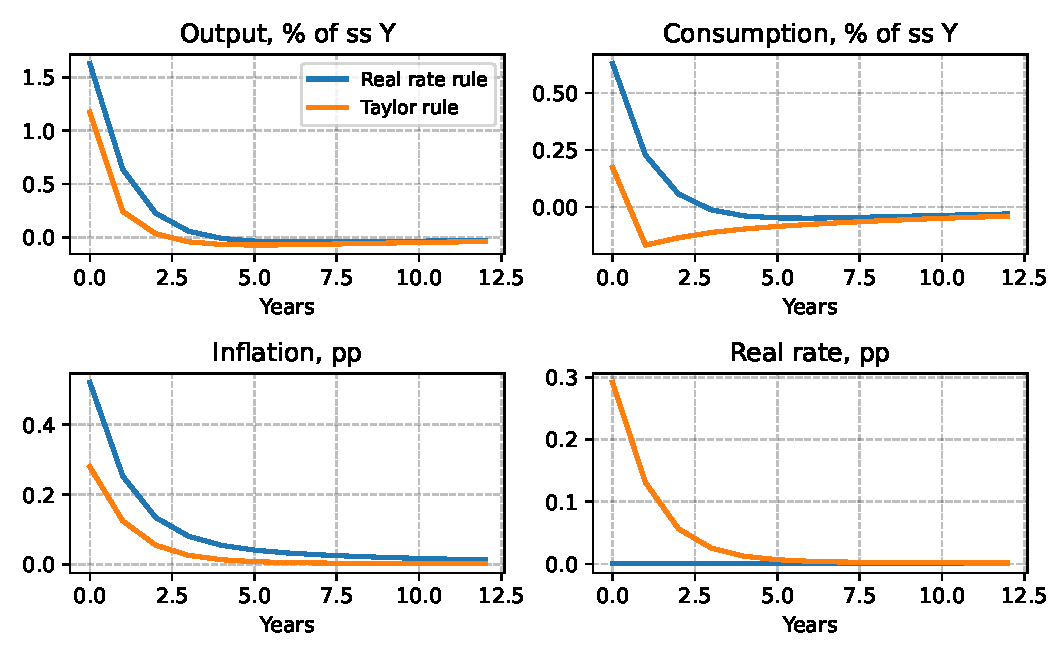
\includegraphics[width=0.68\linewidth]{figs/HANK_G_taylor.pdf}
\end{figure}
\item <+->$G$ raises demand, so wages and inflation rise. The Taylor rule raises $r$, which crowds out $C$
\item <+->Impact multiplier falls from 1.63 to 1.17, cumulative from 1.23 to 0.43
\end{itemize}
\end{frame}
%
\begin{frame}{3. Nominal bonds}
\vspace{-1mm}
\begin{itemize}
\item <+->Back to $\mu=1$ and the real rate rule, now with nominal bonds
\item <+->\textbf{Surprise inflation} lowers the return on debt at $t=0$ only: $dr_{0}^{b}\approx-(1+r_{ss})d\pi_{0}$
\item <+->\textbf{Bondholders lose:} $\text{cap}_{0}=B_{ss}dr_{0}^{b}$
\item <+->\textbf{Taxpayers gain:} the government pays less at $t=0$, with $\boldsymbol{e}_{0}$ the first unit vector:
\[
d\boldsymbol{T}=d\boldsymbol{G}-\left(\boldsymbol{I}-(1+r_{ss})\boldsymbol{L}\right)d\boldsymbol{B}+\boldsymbol{e}_{0}B_{ss}dr_{0}^{b}
\]
\item <+->\textbf{IKC:} with $d\boldsymbol{T}^{real}$ the taxes under real bonds,
\[
d\boldsymbol{Y}=d\boldsymbol{G}+\boldsymbol{M}\left(d\boldsymbol{Y}-d\boldsymbol{T}^{real}\right)+\left(\boldsymbol{m}-\boldsymbol{M}\boldsymbol{e}_{0}\right)B_{ss}dr_{0}^{b}
\]
\item <+->Inflation redistributes from savers (iMPCs $\boldsymbol{m}$) to taxpayers (iMPCs $\boldsymbol{M}\boldsymbol{e}_{0}$, higher): demand rises
\item <+->The deficit no longer has zero present value: $\boldsymbol{q}^{\prime}(d\boldsymbol{G}-d\boldsymbol{T})=-B_{ss}dr_{0}^{b}>0$. Inflation pays part of it
\item <+->$d\pi_{0}$ comes from the W-NKPC, so again two vector equations
\end{itemize}
\end{frame}
%
\begin{frame}{All together}
\vspace{-2mm}
{\small
\begin{align*}
\text{Goods:}\quad & d\boldsymbol{Y}=d\boldsymbol{G}+\bar{\boldsymbol{M}}\left(d\boldsymbol{Y}-d\boldsymbol{T}\right)+\bar{\boldsymbol{M}}^{r}d\boldsymbol{r}+\boldsymbol{m}B_{ss}dr_{0}^{b}\\
\text{W-NKPC:}\quad & d\boldsymbol{\pi}=\boldsymbol{K}\left(\nu d\boldsymbol{Y}+\frac{\sigma}{C_{ss}}\left(d\boldsymbol{Y}-d\boldsymbol{G}\right)+\frac{d\boldsymbol{\tau}}{1-\tau_{ss}}\right)\\
\text{Rates:}\quad & d\boldsymbol{r}=\left(\phi\boldsymbol{I}-(1+r_{ss})\boldsymbol{F}\right)d\boldsymbol{\pi},\quad dr_{0}^{b}\approx-(1+r_{ss})d\pi_{0}\\
\text{Taxes:}\quad & d\boldsymbol{T}=d\boldsymbol{G}-\left(\boldsymbol{I}-(1+r_{ss})\boldsymbol{L}\right)d\boldsymbol{B}+B_{ss}\left(\boldsymbol{L}d\boldsymbol{r}+\boldsymbol{e}_{0}dr_{0}^{b}\right)
\end{align*}
}
\begin{itemize}
\item <+->$\bar{\boldsymbol{M}}^{r}\equiv\boldsymbol{M}^{r}-\frac{p}{1+r_{ss}}\boldsymbol{m}\boldsymbol{q}^{\prime}$: a higher $r$ also lowers stock prices
\item <+->Solving this gives the same $d\boldsymbol{Y}$ and $d\boldsymbol{\pi}$ as the full model
\item <+->An active Taylor rule lowers the multiplier, and nominal bonds raise it
\item <+->A fixed rate at the ZLB also raises it (Christiano et al., 2011)
\end{itemize}
\end{frame}
%

\section{Unions}

\begin{frame}{Why sticky wages instead of sticky prices?}
\begin{itemize}
\item <+->Same $Y$ and $\pi$ for monetary and fiscal shocks: same Phillips curve slope in output
\item <+->Firms become trivial
\item <+->In the data profits are \emph{pro-cyclical}. With sticky prices, wages rise more than prices in a boom, so profits fall. With sticky wages, they do not\\
\begin{figure}[H]
\centering
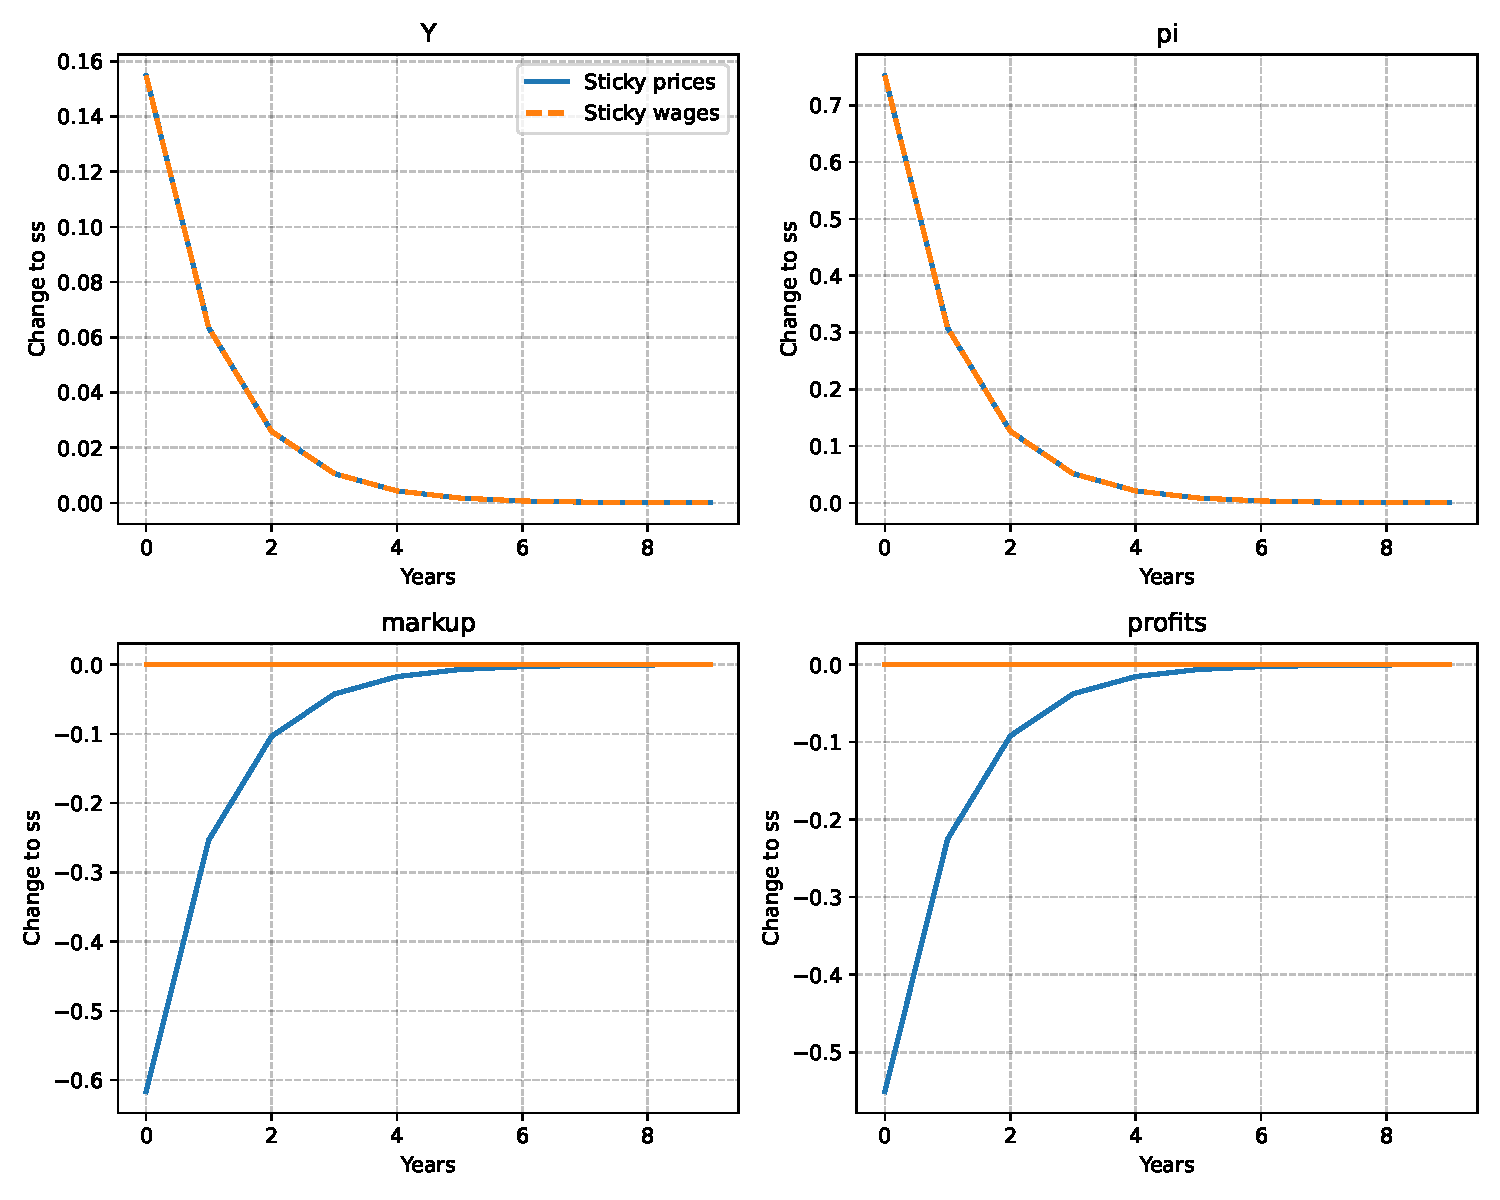
\includegraphics[width=0.5\linewidth]{figs/monpol_irf_sticky_w_p.pdf}
\end{figure}
\end{itemize}
\end{frame}
%
\begin{frame}{Flexible wages and MPCs}
\begin{itemize}
\item <+->Textbook NK model features \textbf{sticky} prices\textbf{, flexible}
wages
\begin{itemize}
\item Fine for some questions, but can cause issues in HA models (see Auclert,
Bardóczy, and Rognlie (2023))
\end{itemize}
\item <+->\textbf{EX}: Standard HA model where households have flexible
labor supply with FOC (EIS=1,Frisch=1):
\begin{align*}
u'\left(c_{i}\right)= & h'\left(l_{i}\right)\\
\Leftrightarrow c_{i}^{-1}=\varphi & l_{i}
\end{align*}
\item <+->What happens if we give household $i$ a lumpsum transfer $\chi$?
\begin{align*}
-c_{i}^{-2}\frac{\partial c_{i}}{\partial\chi}=\varphi & \frac{\partial l_{i}}{\partial\chi}
\end{align*}
\item <+->Define $MPC_{i}=\frac{\partial c_{i}}{\partial\chi},MPE_{i}=-\frac{\partial l_{i}}{\partial\chi}$
as the change in consumption and change in earnings following transfer:
\[
MPC_{i}=\frac{c_{i}}{l_{i}}MPE_{i}
\]
\item <+->If HHs have little saving, $c_{i}\approx l_{i}$ $\Rightarrow$
$MPC_{i}=MPE_{i}$!
\end{itemize}
\end{frame}
%
\begin{frame}{Why unions: MPCs and MPEs}
\begin{itemize}
\item <+->HA model with flexible labor supply implies a tight link between $MPC_{i}$ and $MPE_{i}$
\item <+->\textbf{MPCs in the data}: annual estimates between 0.3 and 0.7
\item <+->\textbf{MPEs in the data}: range from 0 to 0.04 annually
\item <+->So high MPCs imply far too large wealth effects on labor supply
\item <+->\textbf{Solution:} unions take households off their labor supply curves
\begin{itemize}
\item Households do not choose $l_{it}$
\item Wealth effects on aggregate $L$ are small, and sticky wages dampen them further
\end{itemize}
\end{itemize}
\end{frame}

\begin{frame}{Exercise: fiscal policy in HANK}
The code is in \emph{Exercise-HANK}; \emph{model\_type} switches between the two models. Shock: $dG$ with $dB_{t}=\rho_{B}(dB_{t-1}+dG_{t})$.\\
\textbf{IKC model} (\emph{model\_type = 'IKC'}):
\begin{enumerate}
\item {\small Solve for $d\boldsymbol{Y}$ with the IKC equation. Compare with \emph{model.find\_IRFs()}.}
\item {\small Compute the impact and cumulative multipliers for $\rho_{B}\in\{0.8,0.85,0.9,0.95,0.99\}$. Explain.}
\end{enumerate}
\textbf{Canonical model} (\emph{model\_type = 'canonical'}):
\begin{enumerate}
\setcounter{enumi}{2}
\item {\small Same multipliers with capital gains and a Taylor rule. Compare with the IKC model.}
\item {\small Multipliers for $\phi_{\pi}\in\{1.01,1.25,1.5\}$. How does the central bank affect the multiplier?}
\item {\small Same question with $\kappa\in\{0.08,0.16,0.32\}$.}
\item {\small Add nominal bonds. How does $r_{0}^{p}$ react on impact?}
\item {\small Calibrate the share of patient households to an annual MPC of 0.5. How do the multipliers change?}
\end{enumerate}
\end{frame}
%

\section{Summary}

\begin{frame}{Fiscal policy in HANK: literature}
\begin{itemize}
\item Seminal paper:\textbf{ Intertemporal Keynesian Cross}; survey: Auclert, Rognlie and Straub (2025)
\item \textbf{Many} other interesting papers:
\item McKay and Reis - \emph{The role of automatic stabilizers in the US
business cycle} (2016)
\begin{itemize}
\item Analyze the role of automatic stabilizers in a HANK model
\end{itemize}
\item Bayer, Born, Luetticke - \emph{The liquidity channel of fiscal policy}
(2023)
\begin{itemize}
\item Role of liquid and illiquid effects of fiscal policy
\end{itemize}
\item Hagedorn, Manovskii, and Mitman - \emph{The fiscal multiplier} (2019)
\begin{itemize}
\item Systematic evaluation of multiplier in HANK + ZLB
\end{itemize}
\item Druedahl, Ravn, Sunder-Plassmann, Sundram, \& Waldstrøm - \emph{Fiscal
Multipliers in Small Open Economies With Heterogeneous Households
(2024)}
\begin{itemize}
\item Generalize to small open economies
\end{itemize}
\end{itemize}
\end{frame}
%
\begin{frame}{References cited in the lecture}
\small
\begin{itemize}
\item Angeletos, Lian and Wolf - \emph{Can deficits finance themselves?} (2024)
\item Auclert, Bardóczy and Rognlie - \emph{MPCs, MPEs, and multipliers: a trilemma for New Keynesian models} (2023)
\item Christiano, Eichenbaum and Rebelo - \emph{When is the government spending multiplier large?} (2011)
\item Erceg, Henderson and Levin - \emph{Optimal monetary policy with staggered wage and price contracts} (2000)
\item Fagereng, Holm and Natvik - \emph{MPC heterogeneity and household balance sheets} (2021)
\item Galí - \emph{Monetary Policy, Inflation, and the Business Cycle}, ch. 3-4
\item Kaplan, Moll and Violante - \emph{Monetary policy according to HANK} (2018)
\item Ramey - \emph{Ten years after the financial crisis: what have we learned from the renaissance in fiscal research?} (2019)
\end{itemize}
\end{frame}
%
\begin{frame}{Summary and next week}
\begin{itemize}
\item \textbf{Today:}
\begin{itemize}
\item Same macro blocks, three household blocks, one object $\boldsymbol{M}$
\item RANK: deficits are neutral. TANK: amplification on impact only. HANK: larger and more persistent
\end{itemize}
\item \textbf{Next week: }Assignment workshop
\item \textbf{Homework:}
\begin{enumerate}
\item Work on exercise
\item Work on assignment
\end{enumerate}
\end{itemize}
\end{frame}
%

\end{document}
